% 第 6 章 前推与拉回
\chapter{前推与拉回}

本章我们引入两个极其重要的概念：向量的\newterm{push-forward}{前推}{push-forward}与微分形式的\newterm{pull-back}{拉回}{pull-back}. 在第 1 节我们仔细考察一个简单的\newterm{coordinate-transformation}{坐标变换}{coordinate transformation}，看看这个坐标变换对单位正方形的体积有什么影响. 这使我们在第 2 节能够引出向量的前推. 向量的前推使我们能够把向量从一个流形移动，或者说"前推"，到另一个流形. 在坐标变换的情形下，两个流形实际上是同一个流形，只是配备了不同的坐标系.

利用微分形式吃进向量这一事实，我们在第 3 节用向量的前推来定义微分形式的拉回，其中我们把一个流形上的微分形式"拉回"到另一个流形. 同样，在坐标变换的情形下，两个流形实际上真的是同一个流形，只是配备了不同的坐标系. 然后我们更仔细地考察\newterm{volume-form}{体积形式}{volume form}的拉回，它在第 3 节的积分问题中起着至关重要的作用. 我们能够为体积形式的拉回导出一个漂亮的公式，其中包含坐标变换的 Jacobian 矩阵.

然后我们利用前推与拉回仔细考察一些熟悉的例子. 极坐标在第 4 节讨论，柱坐标与球坐标在第 5 节讨论. 第 6 节我们考虑非体积形式的微分形式的拉回，最后在第 7 节我们证明三个恒等式，它们对我们做涉及拉回的计算至关重要.

\section{坐标变换：线性例子}

本节是我们对坐标变换的初次考察. 我们不打算在本节做到完全严谨，这实际上只是想让我们对大局看得更清楚一些. 在我们开始摆弄漂亮的极坐标和球坐标之前，让我们考虑一个简单的情形. 坐标变换无非是 $\mathbb{R}^n$ 与 $\mathbb{R}^n$ 之间既是单射又是满射的映射. 由于 $\mathbb{R}^n$ 与 $\mathbb{R}^n$ 相同，我们常常把它想成 $\mathbb{R}^n$ 到自身的映射. 考虑由
\[
u(x,y)=x+y,\qquad v(x,y)=x-y
\]
给出的两个映射 $u,v:\mathbb{R}^2\to\mathbb{R}^2$.

图~\ref{fig:6-1} 显示了这个坐标变换. 左边是用 $xy$ 坐标表示的 $\mathbb{R}^2$，我们也把它称为 $xy$ 平面或 $\mathbb{R}^2_{xy}$；右边是用 $uv$ 坐标表示的 $\mathbb{R}^2$，我们也把它称为 $uv$ 平面或 $\mathbb{R}^2_{uv}$. 所以，即使 $\mathbb{R}^2$ 就是 $\mathbb{R}^2$，我们也根据所用的坐标对这两个副本作出区分. 在左上角，来自 $xy$ 平面的 $x$ 网格线与 $y$ 网格线被映射到右边 $uv$ 平面上的直线；在右下角，$u$ 网格线与 $v$ 网格线被映射到左边 $xy$ 平面上的直线.

\begin{figure}[htbp]
  \centering
  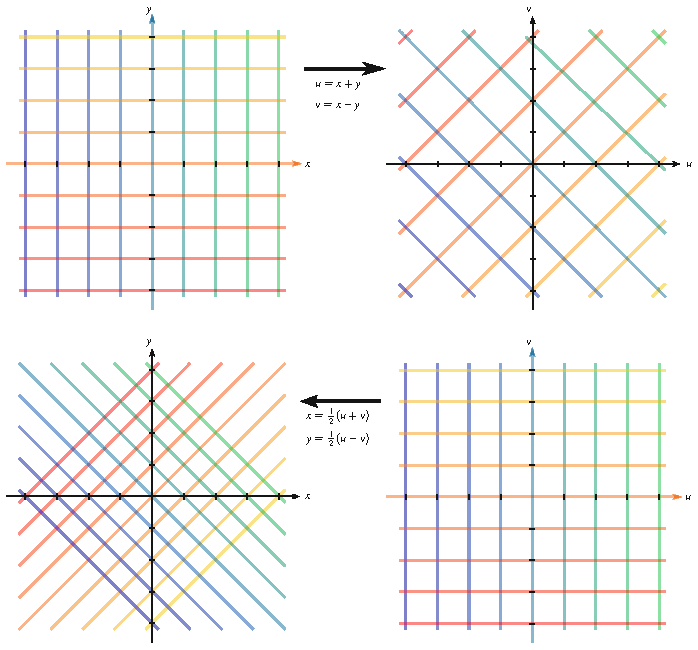
\includegraphics[width=0.960\linewidth]{images/vector/fig-6-1.pdf}
  \caption{平面 $\mathbb{R}^2_{xy}$（左）与 $\mathbb{R}^2_{uv}$（右）. 由 $u(x,y)=x+y$ 与 $v(x,y)=x-y$ 给出的坐标变换位于顶部（从左到右）. 逆坐标变换 $x(u,v)=\frac12(u+v)$ 与 $y(u,v)=\frac12(u-v)$ 位于底部（从右到左）. 颜色编码显示了各条直线是如何映射的}
  \label{fig:6-1}
\end{figure}

\begin{question}\label{q:6-1}
求下列直线在映射 $u=x+y$ 与 $v=x-y$ 下的像，并把你求出的结果与图~\ref{fig:6-1} 顶部所示的映射进行比较.
\begin{enumerate}
  \item[(a)] $x=0$
  \item[(b)] $x=1$
  \item[(c)] $x=4$
  \item[(d)] $y=0$
  \item[(e)] $y=1$
  \item[(f)] $y=-3$
\end{enumerate}
\end{question}

\begin{question}\label{q:6-2}
求下列直线在逆映射 $x=\frac12(u+v)$ 与 $y=\frac12(u-v)$ 下的像，并把你求出的结果与图~\ref{fig:6-1} 底部所示的映射进行比较.
\begin{enumerate}
  \item[(a)] $u=0$
  \item[(b)] $u=1$
  \item[(c)] $u=4$
  \item[(d)] $v=0$
  \item[(e)] $v=1$
  \item[(f)] $v=-3$
\end{enumerate}
\end{question}

我们用坐标函数 $u=x+y$ 与 $v=x-y$ 把平面 $\mathbb{R}^2_{xy}$ 中的点映射为 $\mathbb{R}^2_{uv}$ 中的点，如下所示：
\[
\begin{array}{lcl}
(x,y)&\longrightarrow&(x+y,x-y)=(u,v)\\
(0,0)&\longrightarrow&(0+0,0-0)=(0,0)\\
(1,0)&\longrightarrow&(1+0,1-0)=(1,1)\\
(1,1)&\longrightarrow&(1+1,1-1)=(2,0)\\
(0,1)&\longrightarrow&(0+1,0-1)=(1,-1).
\end{array}
\]
当我们在 $\mathbb{R}^2_{xy}$ 中绕着单位正方形移动时，可以跟踪 $\mathbb{R}^2_{uv}$ 中发生的情况：
\[
\begin{array}{ll}
(x,y):&(0,0)\longrightarrow(1,0)\longrightarrow(1,1)\longrightarrow(0,1)\longrightarrow(0,0)\\
(u,v):&(0,0)\longrightarrow(1,1)\longrightarrow(2,0)\longrightarrow(1,-1)\longrightarrow(0,0).
\end{array}
\]

由此我们可以看到，如图~\ref{fig:6-2} 所示，来自 $xy$ 坐标的单位正方形被映射为 $uv$ 坐标中的菱形. 注意，当你沿着图~\ref{fig:6-2} 左边所示的 $xy$ 坐标中的单位正方形以逆时针方向移动时，你是在沿着图~\ref{fig:6-2} 右边所示的 $uv$ 坐标中的菱形以顺时针方向移动. 还有另一个有趣的差别. 考虑 $xy$ 平面中单位正方形的面积，它的面积是 $1$；而 $uv$ 平面中菱形的面积，即单位正方形的像，其面积是 $2$.

\begin{figure}[htbp]
  \centering
  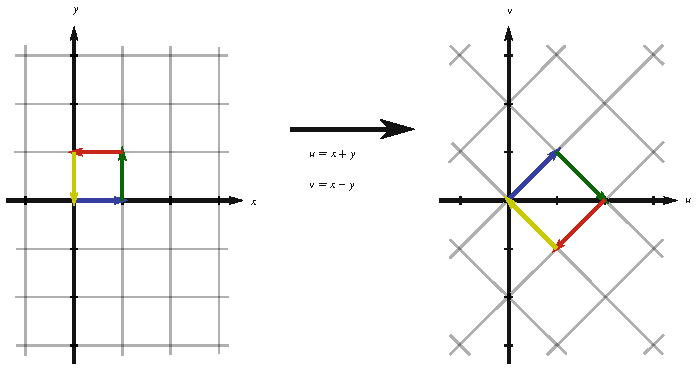
\includegraphics[width=0.960\linewidth]{images/vector/fig-6-2.pdf}
  \caption{$\mathbb{R}^2_{xy}$ 中的单位正方形（左）被映射为 $\mathbb{R}^2_{uv}$ 中的菱形（右）. 注意定向从逆时针变为顺时针，面积从 1 增加到 2}
  \label{fig:6-2}
\end{figure}

\begin{figure}[htbp]
  \centering
  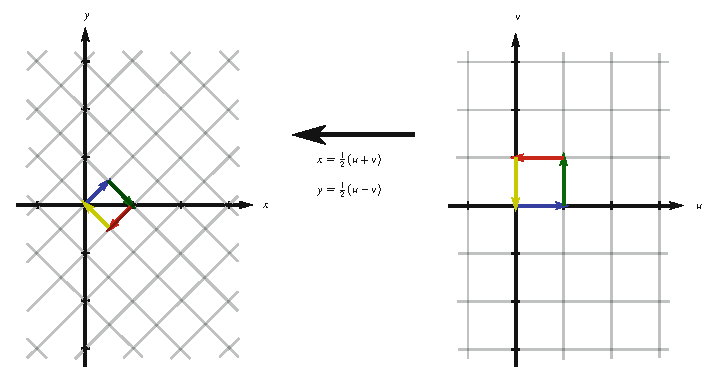
\includegraphics[width=0.960\linewidth]{images/vector/fig-6-3.pdf}
  \caption{$\mathbb{R}^2_{uv}$ 中的单位正方形（右）被映射为 $\mathbb{R}^2_{xy}$ 中的菱形（左）. 注意定向从逆时针变为顺时针，面积从 1 减小到二分之一}
  \label{fig:6-3}
\end{figure}

\begin{question}\label{q:6-3}
证明在逆映射 $x=\frac12(u+v)$ 与 $y=\frac12(u-v)$ 下点 $(0,0)$、$(1,0)$、$(1,1)$ 和 $(0,1)$ 会怎样.
\end{question}

类似地，如果我们用逆映射把来自 $uv$ 坐标平面（如图~\ref{fig:6-3} 右边所示）的单位正方形送到 $xy$ 坐标平面，那么我们在 $xy$ 坐标平面中得到一个菱形（如图~\ref{fig:6-3} 左边所示），其面积为原来的一半且方向反转. 接下来注意到
\[
dx\wedge dy\underbrace{\left(\binom{1}{0}_{xy(0,0)},\binom{0}{1}_{xy(0,0)}\right)}_{\text{xy 平面中的向量}}=\left|\begin{matrix}1&0\\0&1\end{matrix}\right|=1,
\]
以及
\[
du\wedge dv\underbrace{\left(\binom{1}{0}_{uv(0,0)},\binom{0}{1}_{uv(0,0)}\right)}_{\text{uv 平面中的向量}}=\left|\begin{matrix}1&0\\0&1\end{matrix}\right|=1,
\]
所以 $dx\wedge dy$ 是 $xy$ 平面的\newterm{area-form}{面积形式}{area form}，而 $du\wedge dv$ 是 $uv$ 平面的面积形式.

首先我们把 $du\wedge dv$ 写成 $dx\wedge dy$ 的形式. 其中一部分已经完成了. 由于 $u=x+y$ 与 $v=x-y$，我们有
\[
du=d(x+y)=dx+dy,\qquad dv=d(x-y)=dx-dy
\]
所以我们有
\begin{align*}
du\wedge dv&=(dx+dy)\wedge(dx-dy)\\
&=dx\wedge(dx-dy)+dy\wedge(dx-dy)\\
&=dx\wedge dx-dx\wedge dy+dy\wedge dx-dy\wedge dy\\
&=-dx\wedge dy-dx\wedge dy\\
&=-2dx\wedge dy.
\end{align*}

接下来我们把 $dx\wedge dy$ 写成 $du\wedge dv$ 的形式. 在上面的问题~\ref{q:6-3}中你证明了，用 $u$ 和 $v$ 解出 $x$ 和 $y$ 得到
\[
x=\frac12(u+v),\qquad y=\frac12(u-v)
\]
这反过来又给出
\[
dx=d\left(\frac12(u+v)\right)=\frac12du+\frac12dv,\qquad
dy=d\left(\frac12(u-v)\right)=\frac12du-\frac12dv
\]
所以我们有
\begin{align*}
dx\wedge dy&=\left(\frac12du+\frac12dv\right)\wedge\left(\frac12du-\frac12dv\right)\\
&=\frac14dv\wedge du-\frac14du\wedge dv\\
&=-\frac12du\wedge dv.
\end{align*}
总而言之，我们刚才所做的就是计算 $xy$ 面积形式与 $uv$ 面积形式之间的下列关系
\[
du\wedge dv=-2dx\wedge dy,\qquad dx\wedge dy=-\frac12du\wedge dv.
\]

把图~\ref{fig:6-2} 与图~\ref{fig:6-3} 中发生的事情与面积形式之间的关系进行比较. 它们彼此之间有什么关系？首先，我们尝试理解体积形式的关系告诉我们什么. 首先考虑图~\ref{fig:6-2}，其中 $xy$ 平面中的单位正方形被映射为 $uv$ 平面中的菱形. $uv$ 平面中菱形的体积是 $xy$ 平面中单位正方形体积的 $-2$ 倍. 我们可以看出 2 从何而来：注意到 $xy$ 平面中的单位正方形被映射为面积是其两倍的 $uv$ 平面中的菱形. 那么负号又从何而来？来自注意到 $xy$ 平面中的逆时针旋转变成了 $uv$ 平面中的顺时针旋转. 这就是我们的有向体积. 所以，我们所展示的必然与恒等式
\[
du\wedge dv=-2dx\wedge dy
\]
有某种关系.

接下来考虑图~\ref{fig:6-3}，其中 $uv$ 平面中的单位正方形被映射为 $xy$ 平面中的菱形. $xy$ 平面中菱形的面积是 $uv$ 平面中单位正方形体积的 $-\frac12$ 倍. 这意味着 $uv$ 平面中（有向）体积为 1 的单位正方形被映射为 $xy$ 平面中（有向）体积为 $-\frac12$ 的菱形，其中负号再次表明，绕着 $uv$ 平面中正方形的逆时针旋转变成了绕着 $xy$ 平面中菱形的顺时针旋转. 同样，这显然与恒等式
\[
dx\wedge dy=-\frac12du\wedge dv
\]
有某种关系.

回想一下，当我们在第 1.2 节推导行列式的公式时，我们一开始规定了我们认为体积应当具有的三个基本而直观的性质：
\begin{enumerate}
  \item 单位立方体的体积应为 1（在任何维数下）.
  \item 退化的平行六面体（即 $\mathbb{R}^n$ 中小于 $n$ 维的平行六面体）的 $n$ 维体积应为零.
  \item 把一条边缩放 $c$ 倍，体积应改变 $c$ 倍.
\end{enumerate}
通过假设我们的体积函数 $D$ 只具有这三个性质，我们发现了第四个性质：交换（对调）平行六面体的两条边也会改变体积的符号. 换句话说，在我们对体积的直观认识中，最基本的是\newterm{orientation}{定向}{orientation}的概念. 在三维中，定向常常被伪装成"右手法则". 见图~\ref{fig:6-4}.

\begin{figure}[htbp]
  \centering
  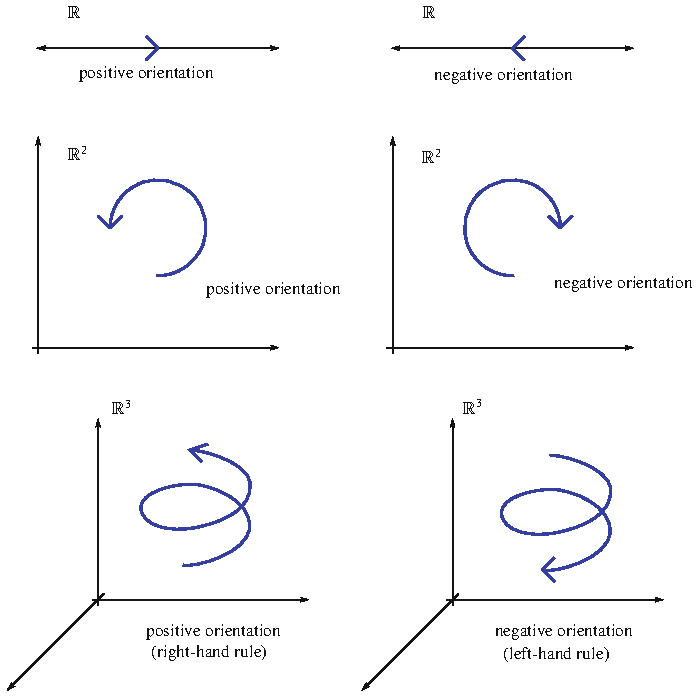
\includegraphics[width=0.829\linewidth]{images/vector/fig-6-4.pdf}
  \caption{$\mathbb{R}$（顶部）、$\mathbb{R}^2$（中部）与 $\mathbb{R}^3$（底部）的两种定向}
  \label{fig:6-4}
\end{figure}

在过去的几页中我们一直有点不严谨，但至少现在你可能开始看到，不同坐标系中的这些体积形式是如何相互关联的——当你从一个坐标系移动到另一个坐标系时，它们以某种方式编码了体积的变化. 这正是我们在积分时换元时会用到的那类东西.

现在我们想更仔细地考察体积形式. $xy$ 平面中的单位正方形由 $xy$ 平面中的向量
\[
\binom{1}{0}_{xy(0,0)},\qquad\binom{0}{1}_{xy(0,0)}
\]
给出（张成）. 换句话说，由这两个向量张成的平行六面体就是单位正方形. 这里我们在下标中用 $xy$ 表示这些向量所在的坐标平面. 这些向量在坐标变换 $u=x+y$ 与 $v=x-y$ 下的投影由
\[
\binom{1}{0}_{xy(0,0)}\longmapsto\binom{1}{1}_{uv(0,0)},\qquad
\binom{0}{1}_{xy(0,0)}\longmapsto\binom{1}{-1}_{uv(0,0)}
\]
给出. 见图~\ref{fig:6-5}. 容易计算出
\begin{align*}
dx\wedge dy\left(\binom{1}{0}_{xy(0,0)},\binom{0}{1}_{xy(0,0)}\right)=\left|\begin{matrix}1&0\\0&1\end{matrix}\right|=1, \\
du\wedge dv\left(\binom{1}{1}_{uv(0,0)},\binom{1}{-1}_{uv(0,0)}\right)=\left|\begin{matrix}1&1\\1&-1\end{matrix}\right|=-2.
\end{align*}

\begin{figure}[htbp]
  \centering
  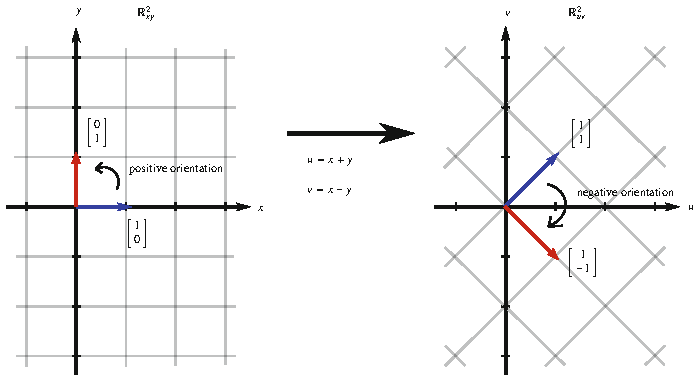
\includegraphics[width=0.960\linewidth]{images/vector/fig-6-5.pdf}
  \caption{$xy$ 平面中的基向量被映射为 $uv$ 平面中的两个向量. 注意定向发生变化}
  \label{fig:6-5}
\end{figure}

回想面积形式会求输入向量张成的平行六面体的面积，这与我们从图中预期的完全一致. 我们也开始对恒等式
\[
dx\wedge dy=-\frac12du\wedge dv
\]
的含义有了更清晰的图景. 实际上我们有
\[
dx\wedge dy\left(\binom{1}{0}_{xy(0,0)},\binom{0}{1}_{xy(0,0)}\right)
=-\frac12du\wedge dv\left(\binom{1}{1}_{uv(0,0)},\binom{1}{-1}_{uv(0,0)}\right).
\]
面积形式 $dx\wedge dy$ 必须吃进来自 $xy$ 平面的向量，而面积形式 $du\wedge dv$ 必须吃进来自 $uv$ 平面的向量. 此外，面积形式 $du\wedge dv$ 所吃进的向量，正是面积形式 $dx\wedge dy$ 所吃进的向量在映射 $u$ 与 $v$（$u=x+y$ 与 $v=x-y$）下的投影.

类似地，$uv$ 平面中的单位正方形由向量
\[
\binom{1}{0}_{uv(0,0)},\qquad\binom{0}{1}_{uv(0,0)}
\]
张成. 在上述坐标变换的逆变换 $x=\frac12(u+v)$ 与 $y=\frac12(u-v)$ 下，这些向量的投影由
\[
\binom{1}{0}_{uv(0,0)}\longmapsto\binom{1/2}{1/2}_{xy(0,0)},\qquad
\binom{0}{1}_{uv(0,0)}\longmapsto\binom{1/2}{-1/2}_{xy(0,0)}
\]
给出. 见图~\ref{fig:6-6}. 同样，容易计算出
\begin{align*}
du\wedge dv\left(\binom{1}{0}_{uv(0,0)},\binom{0}{1}_{uv(0,0)}\right)=\left|\begin{matrix}1&0\\0&1\end{matrix}\right|=1, \\
dx\wedge dy\left(\binom{1/2}{1/2}_{xy(0,0)},\binom{1/2}{-1/2}_{xy(0,0)}\right)=\left|\begin{matrix}1/2&1/2\\1/2&-1/2\end{matrix}\right|=-\frac12.
\end{align*}

\begin{figure}[htbp]
  \centering
  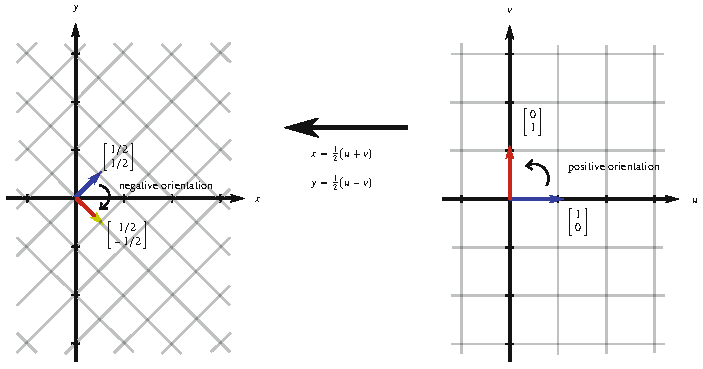
\includegraphics[width=0.960\linewidth]{images/vector/fig-6-6.pdf}
  \caption{$uv$ 平面中的基向量被映射为 $xy$ 平面中的两个向量. 注意定向发生变化}
  \label{fig:6-6}
\end{figure}

这同样与我们从图中预期的完全一致. 而且，我们开始更好地理解恒等式
\[
du\wedge dv=-2dx\wedge dy
\]
实际上是如何成立的：
\[
du\wedge dv\left(\binom{1}{0}_{uv(0,0)},\binom{0}{1}_{uv(0,0)}\right)
=-2dx\wedge dy\left(\binom{1/2}{1/2}_{xy(0,0)},\binom{1/2}{-1/2}_{xy(0,0)}\right).
\]
面积形式 $du\wedge dv$ 吃进来自 $uv$ 平面的向量，而面积形式 $dx\wedge dy$ 吃进来自 $xy$ 平面的向量. 此外，$dx\wedge dy$ 所吃进的向量，正是 $du\wedge dv$ 所吃进的向量在映射 $x$ 与 $y$（$x=\frac12(u+v)$ 与 $y=\frac12(u-v)$）下的投影. 所以我们的恒等式
\[
du\wedge dv=-2dx\wedge dy,\qquad dx\wedge dy=-\frac12du\wedge dv
\]
成立，但仅当它们所吃进的向量之间存在特定的关系时，也就是说，当它们所吃进的向量由两个空间之间的映射相关联时.

当然，在本节中我们犯了向量微积分的头号大罪，即把我们上面让体积形式所吃进的各个向量视为流形 $\mathbb{R}^2$ 的一部分，而不是它们实际上所在的 $T_{(0,0)}\mathbb{R}^2$ 的元素. 我们将在下一节纠正这一点. 本节的主要目的是试图更好地理解体积形式之间恒等式所涉及的微妙之处.

\section{向量的前推}

在上一节中我们考察了（线性坐标变换）映射
\[
f(x,y)=\bigl(u(x,y),v(x,y)\bigr):\mathbb{R}^2\to\mathbb{R}^2
\]
其中 $u(x,y)=x+y$ 与 $v(x,y)=x-y$. 然后我们用它们求出了恒等式 $du\wedge dv=-2dx\wedge dy$ 与 $dx\wedge dy=-\frac12du\wedge dv$，并开始探索这些恒等式实际上意味着什么. 它们与定义域流形 $\mathbb{R}^2$（用 $xy$ 坐标，我们记为 $\mathbb{R}^2_{xy}$）中的面积如何关联值域流形 $\mathbb{R}^2$（用 $uv$ 坐标，我们记为 $\mathbb{R}^2_{uv}$）中的面积有关. 我们发现，当 $du\wedge dv$ 所吃进的向量是 $dx\wedge dy$ 所吃进的向量在映射 $f(x,y)=\bigl(u(x,y),v(x,y)\bigr)=(x+y,x-y)$ 下的投影时，恒等式 $du\wedge dv=-2dx\wedge dy$ 成立. 类似地，当我们考虑逆映射时，我们发现当 $dx\wedge dy$ 所吃进的向量是 $du\wedge dv$ 所吃进的向量在逆映射下的投影时，恒等式 $dx\wedge dy=-\frac12du\wedge dv$ 成立. 然而，在这样做的时候，我们对用来确定平行六面体（我们求的是它们的体积）的向量相当不严谨. 如我们所知，向量实际上生活在切空间中，而不在流形中. 正如我们将看到的，我们在这里能够对这一事实一带而过，是因为这个映射是线性的.

并不是想用这个例子把你烦得要死，但在本节中我们将在数学上更精确的同时继续使用这个例子. 这将作为向量的前推这一思想的动机与引入. 在本章后面，这个例子还将作为微分形式的拉回这一思想的动机与引入. 此外，我们也想在引入像极坐标、球坐标或柱坐标这样更复杂的例子之前，先研究一个简单的例子.

接下来我们回想，流形 $\mathbb{R}^2_{xy}$（带 $xy$ 坐标）和流形 $\mathbb{R}^2_{uv}$（带 $uv$ 坐标），见图~\ref{fig:6-1}，在每个点处都有一个切空间，类似于图~\ref{fig:2-15} 所示的情况. 也就是说，如果 $(x,y)$ 是 $\mathbb{R}^2_{xy}$ 中的一个点，那么 $T_{(x,y)}\mathbb{R}^2_{xy}$ 就是 $\mathbb{R}^2_{xy}$ 在点 $(x,y)$ 处的切空间. 点 $f(x,y)=(x+y,x-y)$ 是点 $(x,y)$ 到 $\mathbb{R}^2_{uv}$ 的投影，而 $T_{(x+y,x-y)}\mathbb{R}^2_{uv}$ 是 $\mathbb{R}^2_{uv}$ 在投影点 $(x+y,x-y)$ 处的切空间.

另外，对于映射 $f(x,y)=\bigl(u(x,y),v(x,y)\bigr)=(x+y,x-y)$，$f$ 在点 $(x,y)$ 处的导数由 Jacobian 矩阵 $Df$ 给出：
\[
D_{(x,y)}f=
\begin{bmatrix}
\frac{\partial u}{\partial x}&\frac{\partial u}{\partial y}\\
\frac{\partial v}{\partial x}&\frac{\partial v}{\partial y}
\end{bmatrix}_{(x,y)}.
\]
让我们想一想 Jacobian 矩阵是什么、做什么. 它是函数 $f(x,y)$ 在点 $(x,y)$ 处最接近的线性逼近. 假设我们有某个以点 $(x,y)$ 为基点的向量 $v=\binom{a}{b}$. 这个向量实际上在 $\mathbb{R}^2_{xy}$ 在点 $(x,y)$ 处的切空间中，但暂时我们仍把它想成在流形 $\mathbb{R}^2_{xy}$ 中. 如果我们想知道当我们沿着向量 $v$ 从 $(x,y)$ 移动时 $f$ 改变了多少，我们可以求 $f(x,y)$ 和 $f(x+a,y+b)$ 来看出这一变化. 事实上，我们可以把这一变化想成从 $f(x,y)$ 到 $f(x+a,y+b)$ 的向量. 这里点 $(x,y)$ 和 $(x+a,y+b)$ 都在流形 $\mathbb{R}^2_{xy}$ 中，而点 $f(x,y)$ 和 $f(x+a,y+b)$ 都在流形 $\mathbb{R}^2_{uv}$ 中. 或者我们可以用 $f$ 在点 $(x,y)$ 处最接近的线性逼近来估计这一变化，它就是 $f$ 在点 $(x,y)$ 处的导数，由 Jacobian 矩阵 $Df$ 在点 $(x,y)$ 处给出. 要做到这一点，我们把 Jacobian 矩阵乘以向量 $v$，即求 $Df\cdot v$. 这给出另一个向量. 但这个向量在哪里呢？由于我们是在从点 $f(x,y)$ 处估计 $f$ 的变化，这个点就是我们新向量的基点，所以我们的新向量在 $\mathbb{R}^2_{uv}$ 在点 $f(x,y)$ 处的切空间中. 总而言之，Jacobian 矩阵实际上是一个映射
\[
D_{(x,y)}f:T_{(x,y)}\mathbb{R}^2_{xy}\longrightarrow T_{f(x,y)}\mathbb{R}^2_{uv}.
\]
出于我们稍后将解释的原因，我们通常用记号 $T_{(x,y)}f$ 表示在点 $(x,y)$ 处的 Jacobian 矩阵，而不是更常见的 $D_{(x,y)}f$. 对于我们的特定映射 $f(x,y)=\bigl(u(x,y),v(x,y)\bigr)=(x+y,x-y)$，我们有
\[
T_{(x,y)}f=
\begin{bmatrix}
\frac{\partial u}{\partial x}&\frac{\partial u}{\partial y}\\
\frac{\partial v}{\partial x}&\frac{\partial v}{\partial y}
\end{bmatrix}_{(x,y)}
=
\begin{bmatrix}
1&1\\
1&-1
\end{bmatrix}_{(x,y)}.
\]
例如，在点 $(0,0)$ 处向量 $\binom{1}{0}_{(0,0)}$ 被送到
\[
T_{(0,0)}f\cdot\binom{1}{0}_{(0,0)}
=
\begin{bmatrix}
1&1\\
1&-1
\end{bmatrix}_{(0,0)}
\cdot\binom{1}{0}_{(0,0)}
=
\binom{1}{1}_{f(0,0)=(0,0)},
\]
而向量 $\binom{0}{1}_{(0,0)}$ 被送到
\[
T_{(0,0)}f\cdot\binom{0}{1}_{(0,0)}
=
\begin{bmatrix}
1&1\\
1&-1
\end{bmatrix}_{(0,0)}
\cdot\binom{0}{1}_{(0,0)}
=
\binom{1}{-1}_{f(0,0)=(0,0)}.
\]
所以，从函数
\[
f:\mathbb{R}^2_{xy}\longrightarrow\mathbb{R}^2_{uv},\qquad p\longmapsto f(p)
\]
我们诱导出一个映射
\[
T_pf:T_p\mathbb{R}^2_{xy}\longrightarrow T_{f(p)}\mathbb{R}^2_{uv},\qquad
v_p\longmapsto T_pf\cdot v_p
\]
它从定义域流形 $\mathbb{R}^2_{xy}$ 的切丛到值域流形 $\mathbb{R}^2_{uv}$ 的切丛，无非就是 Jacobian 矩阵. 所谓"诱导"，我们的意思是我们用 $f$ 导出了另一个映射 $Tf$，而当我们把基点 $p$ 也考虑进去时，就得到 $T_pf$. 我们把 $T_pf\cdot v_p$ 称为 $v_p$ 被 $T_pf$ 的前推，而 $T_pf$ 有时被称为前推映射.

我们再做一例. 假设我们想求 $T_pf\cdot v_p$，其中
\[
v_p=\binom{1}{2}_{(1,1)}.
\]
首先我们求 $f(1,1)=(1+1,1-1)=(2,0)$. 接下来有
\[
T_{(1,1)}f\cdot\binom{1}{2}_{(1,1)}
=
\begin{bmatrix}
1&1\\
1&-1
\end{bmatrix}_{(1,1)}
\cdot\binom{1}{2}_{(1,1)}
=
\binom{3}{-1}_{f(1,1)}
=
\binom{3}{-1}_{(2,0)}.
\]
注意左边的基点是 $(1,1)$，而右边的基点是 $f(1,1)=(2,0)$.

\begin{question}\label{q:6-4}
用同一个函数 $f$，求下列向量的 $T_pf\cdot v_p$.
\begin{enumerate}
  \item[(a)] $v_p=\binom{-1}{-1}_{(5,4)}$
  \item[(b)] $v_p=\binom{-2}{3}_{(2,-3)}$
\end{enumerate}
\end{question}

由于 $f$ 已经是线性函数，$f$ 的 Jacobian 矩阵，即映射 $T_pf$，在每个点处都相同. 我们很快就会遇到并非如此的例子. 但还有别的东西值得注意. 考虑一个一般向量 $v_p=\binom{x}{y}_p$. 则
\[
T_pf\cdot\binom{x}{y}_p
=
\begin{bmatrix}
1&1\\
1&-1
\end{bmatrix}_p
\cdot\binom{x}{y}_p
=
\binom{x+y}{x-y}_{f(p)}.
\]
我们有，$T_pf$ 作用于 $\binom{x}{y}_p\in T_p\mathbb{R}^2$（其中 $p\in$ 流形 $\mathbb{R}^2$），看起来与函数 $f$ 作用于 $(x,y)\in$ 流形 $\mathbb{R}^2$ 完全相同：
\[
f(x,y)=(x+y,x-y)\in\mathbb{R}^2,\qquad
T_pf\cdot\binom{x}{y}_p=\binom{x+y}{x-y}_{f(p)}\in T_{f(p)}\mathbb{R}^2,\ p\in\mathbb{R}^2.
\]
当然，$Tf$ 与 $f$ 的定义域和值域是不同的空间，但函数 $Tf$ 与 $f$ 作用于输入点的方式看起来是一样的. 对于线性函数 $f$，你经常会看到人们写下
\[
Tf=f.
\]
显然，由于定义域和值域不同，这在技术上不可能成立，但这是一个方便的所谓"记号的滥用". （实际上，记号的滥用（abuse of notation）在数学中极其常见. 当你最初学习某个东西时，这些记号的滥用常常会妨碍理解，但一旦你理解了正在发生的事情，它们就使计算和记录变得如此简单而快速. 总是绝对精确会让人难以承受，也不必要地困难，而且对真正理解事情的人来说没有必要.）

把我们刚刚学到的东西付诸使用，我们将重做上一节所做的事情. 坚持使用同一个函数 $f(x,y)=\bigl(u(x,y),v(x,y)\bigr)=(x+y,x-y)$，考虑点 $(5,7)\in\mathbb{R}^2_{xy}$. 我们求出 $f(5,7)=(5+7,5-7)=(12,-2)$. 接下来，我们求由该点处的欧几里得单位向量
\[
\binom{1}{0}_{(5,7)},\qquad\binom{0}{1}_{(5,7)}\in T_{(5,7)}\mathbb{R}^2_{xy}
\]
张成的平行六面体的面积. 严格地说，这个平行六面体位于切空间 $T_{(5,7)}\mathbb{R}^2_{xy}$ 中，但鉴于我们可以把切空间与底层的流形 $\mathbb{R}^2_{xy}$ 自然地等同起来，我们常常也把这个平行六面体想成在流形中. 用我们的面积形式 $dx\wedge dy$，我们得到面积为
\[
(dx\wedge dy)_{(5,7)}\left(\binom{1}{0}_{(5,7)},\binom{0}{1}_{(5,7)}\right)=\left|\begin{matrix}1&0\\0&1\end{matrix}\right|=1.
\]
接下来我们用 $T_{(5,7)}f$ 把这些向量前推到空间 $T_{(12,-2)}\mathbb{R}^2_{uv}$：
\begin{align*}
T_{(5,7)}f\cdot\binom{1}{0}_{(5,7)}
=
\begin{bmatrix}
1&1\\
1&-1
\end{bmatrix}
\cdot\binom{1}{0}_{(5,7)}
=
\binom{1}{1}_{(12,-2)}\in T_{(12,-2)}\mathbb{R}^2_{uv}, \\
T_{(5,7)}f\cdot\binom{0}{1}_{(5,7)}
=
\begin{bmatrix}
1&1\\
1&-1
\end{bmatrix}
\cdot\binom{0}{1}_{(5,7)}
=
\binom{1}{-1}_{(12,-2)}\in T_{(12,-2)}\mathbb{R}^2_{uv}.
\end{align*}
现在我们用面积形式 $du\wedge dv$ 求由这些被前推的向量张成的平行六面体的面积：
\[
(du\wedge dv)_{(12,-2)}\left(T_{(5,7)}f\cdot\binom{1}{0}_{(5,7)},T_{(5,7)}f\cdot\binom{0}{1}_{(5,7)}\right)
=\left|\begin{matrix}1&1\\1&-1\end{matrix}\right|=-1-1=-2.
\]
总而言之，对 $p=(5,7)$ 我们求出
\[
(dx\wedge dy)_p\underbrace{\left(\binom{1}{0}_p,\binom{0}{1}_p\right)}_{\text{$T_p\mathbb{R}^2_{xy}$ 中的向量}}=1
\]
以及
\[
(du\wedge dv)_{f(p)}\underbrace{\left(T_pf\cdot\binom{1}{0}_p,T_pf\cdot\binom{0}{1}_p\right)}_{\substack{\text{$T_p\mathbb{R}^2_{xy}$ 中向量的前推，}\\\text{位于 $T_{f(p)}\mathbb{R}^2_{uv}$ 中}}}=-2
\]
把一切结合起来，我们得到如下等式
\[
\underbrace{-2\cdot\underbrace{(dx\wedge dy)_p\left(\binom{1}{0}_p,\binom{0}{1}_p\right)}_{=1}}_{=-2}
=
(du\wedge dv)_{f(p)}\underbrace{\left(T_pf\cdot\binom{1}{0}_p,T_pf\cdot\binom{0}{1}_p\right)}_{=-2}
\]
这正是我们在上一节得到的，只是认识到 $du\wedge dv$ 所吃进的向量是 $dx\wedge dy$ 所吃进的向量的前推. 所以，为了严格地理解恒等式 $-2dx\wedge dy=du\wedge dv$，我们需要处理的概念就是向量的前推.

\begin{question}\label{q:6-5}
考虑同一个坐标变换 $f(x,y)=\bigl(u(x,y),v(x,y)\bigr)=(x+y,x-y)$.
\begin{enumerate}
  \item[(a)] 求 $f(3,-2)$.
  \item[(b)] 求 $(dx\wedge dy)_{(3,-2)}\left(\binom{1}{1}_{(3,-2)},\binom{5}{-1}_{(3,-2)}\right)$.
  \item[(c)] 求 $T_{(3,-2)}f\cdot\binom{1}{1}_{(3,-2)}$ 与 $T_{(3,-2)}f\cdot\binom{5}{-1}_{(3,-2)}$.
  \item[(d)] 求 $(du\wedge dv)_{f(3,-2)}\left(T_{(3,-2)}f\cdot\binom{1}{1}_{(3,-2)},T_{(3,-2)}f\cdot\binom{5}{-1}_{(3,-2)}\right)$.
  \item[(e)] 答案与你从最后一个例子以及关系式 $dx\wedge dy=-\frac12du\wedge dv$ 所预期的一致吗？
\end{enumerate}
\end{question}

现在我们稍微一般化一点，在比我们特定问题更一般的背景下简要考察向量的前推. 考虑两个流形之间的映射 $f:M\to N$. 暂时我们把自己限制在 $M=N=\mathbb{R}^n$（对某个 $n$）的情形. 如果映射 $f=(f_1,f_2,\ldots,f_n)$ 在点 $p\in M$ 处可微（这意味着每个 $f_i$ 都在 $p$ 处可微），且流形 $M$ 的坐标由 $x_1,x_2,\ldots,x_n$ 给出，那么该映射在点 $p\in M$ 处的导数由传统的 Jacobian 矩阵给出：
\[
T_pf=\text{$f$ 在 $p$ 处的 Jacobian 矩阵}
=
\begin{bmatrix}
\frac{\partial f_1}{\partial x_1}\Big|_p&\frac{\partial f_1}{\partial x_2}\Big|_p&\cdots&\frac{\partial f_1}{\partial x_n}\Big|_p\\
\frac{\partial f_2}{\partial x_1}\Big|_p&\frac{\partial f_2}{\partial x_2}\Big|_p&\cdots&\frac{\partial f_2}{\partial x_n}\Big|_p\\
\vdots&\vdots&\ddots&\vdots\\
\frac{\partial f_n}{\partial x_1}\Big|_p&\frac{\partial f_n}{\partial x_2}\Big|_p&\cdots&\frac{\partial f_n}{\partial x_n}\Big|_p
\end{bmatrix}.
\]
由 Jacobian 矩阵给出的映射 $T_pf$ 就是映射 $f:M\to N$ 最接近的线性逼近. 我们已经花了大量时间考虑实值函数 $g:\mathbb{R}^n\to\mathbb{R}$ 与微分 $dg$. 我们知道 $g$ 在点 $p$ 处的微分实际上是 $g$ 在点 $p$ 处最接近的线性逼近. 事实上，我们说过 $dg_p$ 在某种意义上"编码"了 $g$ 在点 $p$ 处的切平面，而当然 $g$ 在点 $p$ 处的切平面就是 $g$ 的图像最接近的线性逼近. 利用笛卡尔坐标，我们可以把 $g$ 的微分写成
\[
dg=\frac{\partial g}{\partial x_1}dx_1+\frac{\partial g}{\partial x_2}dx_2+\cdots+\frac{\partial g}{\partial x_n}dx_n
=\left[\frac{\partial g}{\partial x_1},\frac{\partial g}{\partial x_2},\cdots,\frac{\partial g}{\partial x_n}\right].
\]
在我们的函数 $f=(f_1,f_2,\ldots,f_n)$ 的情形下，每个分量函数 $f_i$ 本身是一个实值函数 $f_i:\mathbb{R}^n\to\mathbb{R}$，因此我们可以分别考虑每个 $f_i$ 的微分：
\begin{align*}
df_1=\frac{\partial f_1}{\partial x_1}dx_1+\frac{\partial f_1}{\partial x_2}dx_2+\cdots+\frac{\partial f_1}{\partial x_n}dx_n
=\left[\frac{\partial f_1}{\partial x_1},\frac{\partial f_1}{\partial x_2},\cdots,\frac{\partial f_1}{\partial x_n}\right], \\
df_2=\frac{\partial f_2}{\partial x_1}dx_1+\frac{\partial f_2}{\partial x_2}dx_2+\cdots+\frac{\partial f_2}{\partial x_n}dx_n
=\left[\frac{\partial f_2}{\partial x_1},\frac{\partial f_2}{\partial x_2},\cdots,\frac{\partial f_2}{\partial x_n}\right], \\
\vdots \\
df_n=\frac{\partial f_n}{\partial x_1}dx_1+\frac{\partial f_n}{\partial x_2}dx_2+\cdots+\frac{\partial f_n}{\partial x_n}dx_n
=\left[\frac{\partial f_n}{\partial x_1},\frac{\partial f_n}{\partial x_2},\cdots,\frac{\partial f_n}{\partial x_n}\right].
\end{align*}
把 $f$ 的各分量函数的余向量与 Jacobian 矩阵的行进行比较. 它们是相同的. 因此，$f$ 的 Jacobian 矩阵的行无非是 $f$ 的各分量函数的微分 $df_i$ 写成行矩阵. Jacobian 矩阵 $Tf$ 是映射 $f:\mathbb{R}^n\to\mathbb{R}^n$ 最接近的线性逼近，因为它的行是每个 $f_i:\mathbb{R}^n\to\mathbb{R}$ 最接近的线性逼近.

\begin{figure}[htbp]
  \centering
  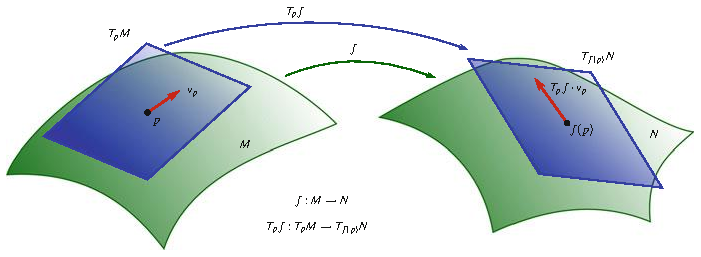
\includegraphics[width=0.960\linewidth]{images/vector/fig-6-7.pdf}
  \caption{映射 $f:M\to N$ 诱导切映射 $Tf:TM\to TN$. 在特定点 $p\in M$ 处我们得到 $T_pf:T_pM\to T_{f(p)}N$. 于是向量 $v_p\in T_pM$ 被前推到向量 $T_pf\cdot v_p\in T_{f(p)}N$}
  \label{fig:6-7}
\end{figure}

和之前一样，假设我们有某个向量 $v_p\in T_pM$. $T_pf\cdot v_p$ 给出当我们沿着 $v_p$ 移动时 $f$ 的变化的线性逼近，它是 $T_{f(p)}N$ 中的另一个向量. 由于我们可以在 $f$ 可微的每个点 $p\in M$ 处求出 $T_pf:T_pM\to T_{f(p)}N$，我们最终得到从 $M$ 的切丛到 $N$ 的切丛的映射 $Tf$. 我们说映射 $f:M\to N$ 诱导映射 $Tf:TM\to TN$. 映射 $Tf$ 把 $T_pM$ 中的向量前推到 $T_{f(p)}N$ 中的向量. 这个映射通常称为由 $f$ 诱导的\newterm{tangent-map}{切映射}{tangent map}. 见图~\ref{fig:6-7}. 我们常常会这样展示，写出类似下面的东西：
\[
\begin{gathered}
TM\xrightarrow{\substack{Tf\\f_*\\Df}}TN\\
v\longmapsto Tf\cdot v\\
M\xrightarrow{f}N\\
p\longmapsto f(p).
\end{gathered}
\]
你会遇到这个诱导映射的三种不同记号：$D_pf$、$T_pf$ 和 $f_*(p)$. $D_pf$ 是相当标准的记号，你会经常遇到它，尤其是在微积分课上. 然而，大概最常用的记号是 $f_*$. 如果我们想包含基点，它常常被写成 $f_*(p)$，这有点笨拙. 这个记号在微分几何书籍中最常遇到. 然而，一般来说我们将使用记号 $Tf$ 或 $T_pf$. 坦白地说，这是一个相当非标准的记号，但我们喜欢它，因为作为一种记号，它包含了大量信息. $Tf$ 中的 $T$ 告诉我们，我们在处理由映射 $f$ 诱导的、从一个切丛到另一个切丛的切映射. 这个记号还可以在我们想要的时候把基点 $p$ 漂亮地包含进去，其方式与切空间记号中包含基点的方式相同. 因此，$T_pf$ 用来指明从切空间 $T_pM$ 到切空间 $T_{f(p)}N$ 的映射.

\section{体积形式的拉回}

在本节中我们将定义体积形式的拉回. 虽然大多数微分形式并不是体积形式，但体积形式在积分中扮演着非常重要的角色，所以我们在本节中将集中于它们. 我们将在后面探讨更一般微分形式的拉回. 目前我们将继续我们的线性例子. 我们的基本目标是把关系式
\[
\underbrace{-2\cdot\underbrace{(dx\wedge dy)_p\left(\binom{1}{0}_p,\binom{0}{1}_p\right)}_{=1}}_{=-2}
=
(du\wedge dv)_{f(p)}\underbrace{\left(T_pf\cdot\binom{1}{0}_p,T_pf\cdot\binom{0}{1}_p\right)}_{=-2}
\]
理解得更精确一些.

回想对于映射 $f(x,y)=(x+y,x-y)$ 我们有
\begin{align*}
du\wedge dv&=d(x+y)\wedge d(x-y)\\
&=(dx+dy)\wedge(dx-dy)\\
&=dx\wedge(dx-dy)+dy\wedge(dx-dy)\\
&=dx\wedge dx-dx\wedge dy+dy\wedge dx-dy\wedge dy\\
&=-dx\wedge dy-dx\wedge dy\\
&=-2dx\wedge dy.
\end{align*}
我们一般性地重做这个计算. 也就是说，考虑由 $f(x,y)=\bigl(u(x,y),v(x,y)\bigr)=(u,v)$ 给出的换元 $f:\mathbb{R}^2_{xy}\to\mathbb{R}^2_{uv}$. 首先我们求
\[
du=\frac{\partial u}{\partial x}dx+\frac{\partial u}{\partial y}dy,\qquad
dv=\frac{\partial v}{\partial x}dx+\frac{\partial v}{\partial y}dy,
\]
然后利用楔积的性质得到
\begin{align*}
du\wedge dv&=\left(\frac{\partial u}{\partial x}dx+\frac{\partial u}{\partial y}dy\right)\wedge\left(\frac{\partial v}{\partial x}dx+\frac{\partial v}{\partial y}dy\right)\\
&=\frac{\partial u}{\partial x}dx\wedge\left(\frac{\partial v}{\partial x}dx+\frac{\partial v}{\partial y}dy\right)
+\frac{\partial u}{\partial y}dy\wedge\left(\frac{\partial v}{\partial x}dx+\frac{\partial v}{\partial y}dy\right)\\
&=\frac{\partial u}{\partial x}\frac{\partial v}{\partial x}\underbrace{dx\wedge dx}_{=0}
+\frac{\partial u}{\partial x}\frac{\partial v}{\partial y}dx\wedge dy
+\frac{\partial u}{\partial y}\frac{\partial v}{\partial x}\underbrace{dy\wedge dx}_{-dx\wedge dy}
+\frac{\partial u}{\partial y}\frac{\partial v}{\partial y}\underbrace{dy\wedge dy}_{=0}\\
&=\frac{\partial u}{\partial x}\frac{\partial v}{\partial y}dx\wedge dy-\frac{\partial u}{\partial y}\frac{\partial v}{\partial x}dx\wedge dy\\
&=\left(\frac{\partial u}{\partial x}\frac{\partial v}{\partial y}-\frac{\partial u}{\partial y}\frac{\partial v}{\partial x}\right)dx\wedge dy\\
&=\underbrace{\left|\begin{matrix}\frac{\partial u}{\partial x}&\frac{\partial u}{\partial y}\\\frac{\partial v}{\partial x}&\frac{\partial v}{\partial y}\end{matrix}\right|}_{\text{Jacobian 矩阵的行列式}}dx\wedge dy.
\end{align*}
本质上看来，当我们在求两个体积形式之间的关系时，Jacobian 矩阵就是"自然而然地蹦出来"的. 在上一节中，我们试图通过引入诱导切映射 $Tf$ 和向量的前推这一思想来更好地理解这个恒等式的含义. 诱导切映射 $Tf$ 按照下式作用：
\[
\begin{gathered}
T_p\mathbb{R}^2\xrightarrow{T_pf}T_{f(p)}\mathbb{R}^2\\
\mathbb{R}^2\xrightarrow{f}\mathbb{R}^2,
\end{gathered}
\]
其中在 $p$ 处的切映射 $T_pf$ 由在 $p$ 处求值的 Jacobian 矩阵给出：
\[
T_pf=
\begin{bmatrix}
\frac{\partial u}{\partial x}&\frac{\partial u}{\partial y}\\
\frac{\partial v}{\partial x}&\frac{\partial v}{\partial y}
\end{bmatrix}_p.
\]
我们把向量 $v_p=\binom{v_1}{v_2}_p\in T_p\mathbb{R}^2$ 的前推定义为
\[
T_pf\cdot v_p=
\begin{bmatrix}
\frac{\partial u}{\partial x}&\frac{\partial u}{\partial y}\\
\frac{\partial v}{\partial x}&\frac{\partial v}{\partial y}
\end{bmatrix}_p
\cdot\binom{v_1}{v_2}_p
=
\begin{bmatrix}
\frac{\partial u}{\partial x}v_1+\frac{\partial u}{\partial y}v_2\\
\frac{\partial v}{\partial x}v_1+\frac{\partial v}{\partial y}v_2
\end{bmatrix}_{f(p)}
\in T_{f(p)}\mathbb{R}^2.
\]
把基点 $p$ 从我们的计算中略去，并在方便之处用 $\det$ 表示行列式，我们有
\begin{align*}
du\wedge dv(Tf\cdot v,Tf\cdot w)
&=\det\begin{bmatrix}du(Tf\cdot v)&du(Tf\cdot w)\\dv(Tf\cdot v)&dv(Tf\cdot w)\end{bmatrix}\\
&=\det\begin{bmatrix}\frac{\partial u}{\partial x}v_1+\frac{\partial u}{\partial y}v_2&\frac{\partial u}{\partial x}w_1+\frac{\partial u}{\partial y}w_2\\[2pt]\frac{\partial v}{\partial x}v_1+\frac{\partial v}{\partial y}v_2&\frac{\partial v}{\partial x}w_1+\frac{\partial v}{\partial y}w_2\end{bmatrix}\\
&=\det\left(\begin{bmatrix}\frac{\partial u}{\partial x}&\frac{\partial u}{\partial y}\\\frac{\partial v}{\partial x}&\frac{\partial v}{\partial y}\end{bmatrix}\begin{bmatrix}v_1&w_1\\v_2&w_2\end{bmatrix}\right)\\
&=\det\begin{bmatrix}\frac{\partial u}{\partial x}&\frac{\partial u}{\partial y}\\\frac{\partial v}{\partial x}&\frac{\partial v}{\partial y}\end{bmatrix}\cdot\det\begin{bmatrix}v_1&w_1\\v_2&w_2\end{bmatrix}\\
&=\left|\begin{matrix}\frac{\partial u}{\partial x}&\frac{\partial u}{\partial y}\\\frac{\partial v}{\partial x}&\frac{\partial v}{\partial y}\end{matrix}\right|\cdot\left|\begin{matrix}dx(v)&dx(w)\\dy(v)&dy(w)\end{matrix}\right|\\
&=\left|\begin{matrix}\frac{\partial u}{\partial x}&\frac{\partial u}{\partial y}\\\frac{\partial v}{\partial x}&\frac{\partial v}{\partial y}\end{matrix}\right|dx\wedge dy(v,w)
\end{align*}
这给我们恒等式
\[
\left|\begin{matrix}\frac{\partial u}{\partial x}&\frac{\partial u}{\partial y}\\\frac{\partial v}{\partial x}&\frac{\partial v}{\partial y}\end{matrix}\right|dx\wedge dy(v,w)
=du\wedge dv(Tf\cdot v,Tf\cdot w).
\]
再次地，当我们计算面积形式在由 $f$ 给出的基变换下如何变化时，Jacobian 矩阵基本上"自然而然地蹦出来了". 但同样，Jacobian 矩阵恰恰就是我们在换基时把向量前推的那个 $Tf$，而向量（或向量的前推）显然是求由向量张成的平行六面体的面积所必需的. 就好像 Jacobian 矩阵在某种意义上"贯穿"了整个计算.

现在我们定义什么是微分形式的拉回. 记住，在本节中我们真正考察过的唯一微分形式就是体积形式，因为它对积分很重要. 但这个基本定义实际上适用于所有微分形式. 假设我们有流形之间的映射 $f:M\to N$. 这个映射诱导切映射 $Tf:TM\to TN$. 现在假设我们在 $N$ 上有一个微分 $k$-形式 $\omega$. 那么我们定义微分 $k$-形式 $T^*f\cdot\omega$ 为 $\omega$ 到 $M$ 的拉回，其中

\begin{definition}[微分形式的拉回]\label{def:6-3-1}
\[
\bigl(T^*f\cdot\omega\bigr)(v_1,v_2,\ldots,v_k)=\omega\bigl(Tf\cdot v_1,Tf\cdot v_2,\ldots,Tf\cdot v_k\bigr).
\]
\end{definition}

这到底想说什么？如果我们给定 $N$（即 $f$ 的值域）上的一个 $k$-形式 $\omega$，那么我们试图求 $M$ 上在某种意义上与 $\omega$"相同"的 $k$-形式. 我们所说的"相同"是什么意思？这两个形式所要吃进的向量来自不同的切空间. 但我们已经知道，$M$ 上的切向量可以用自然的方式前推到 $N$ 上的切向量，所以我们决定利用这一思想. 当我们试图求的 $M$ 上的 $k$-形式吃进 $k$ 个切向量时，我们希望它给出的值，与 $N$ 上的 $k$-形式 $\omega$ 吃进这些同样的向量的前推时给出的值相同. 我们求出的 $M$ 上的这个 $k$-形式记为 $T^*f\cdot\omega$ 或 $f^*\omega$，称为 $\omega$ 的拉回. 最常用的记号是 $f^*$，但出于在切向量的前推那一节中解释过的同样的原因，我们将使用 $T^*f$. 拉回映射有时也称为\newterm{cotangent-map}{余切映射}{cotangent map}.

\begin{figure}[htbp]
  \centering
  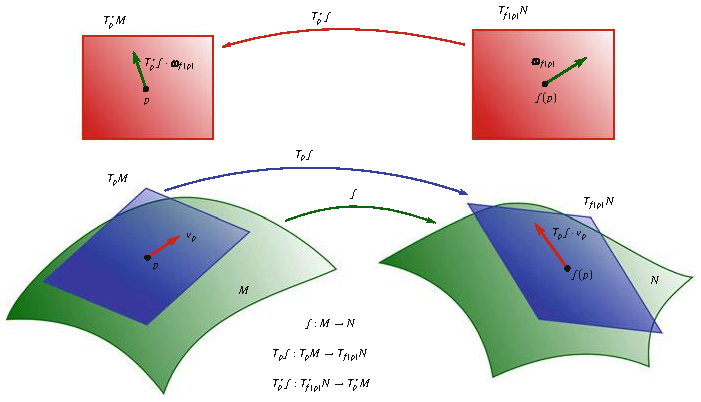
\includegraphics[width=0.960\linewidth]{images/vector/fig-6-8.pdf}
  \caption{映射 $f$ 与 $Tf$ 如图~\ref{fig:6-7} 所示，但现在还包含了拉回映射 $T^*f:T^*N\to T^*M$. 在特定点 $f(p)\in N$ 处我们有 $T_p^*f:T_{f(p)}^*N\to T_p^*M$. 注意映射 $T_p^*f$ 实际上是以值域中的点 $p$ 为下标的. 这相当不寻常，但这样做有助于保持记号一致}
  \label{fig:6-8}
\end{figure}

在这里我们连同基点记号一起展示所有这些映射. 见图~\ref{fig:6-8}. 有一件非常重要的事情值得注意：说到拉回映射，它是按像中的基点而不是定义域中的基点加下标的！这在数学中相当不寻常，但在这种情形下，它恰好是跟踪基点最好的方式. 我们常常把映射 $f$ 及其诱导映射 $T_pf$ 与 $T_p^*f$ 写成
\[
\begin{gathered}
\bigwedge_p^k(M)\xleftarrow{T_p^*f}\bigwedge_{f(p)}^k(N)\\
T_p^*f\cdot\omega_{f(p)}\longleftarrow\omega_{f(p)}\\
T_pM\xrightarrow{T_pf}T_{f(p)}N\\
v_p\longmapsto T_{f(p)}f\cdot v_p\\
M\xrightarrow{f}N\\
p\longmapsto f(p).
\end{gathered}
\]
现在我们准备理解我们的例子中发生的事情. 这里一切都被放在一起：
\[
\underbrace{\left|\begin{matrix}1&1\\1&-1\end{matrix}\right|\cdot(dx\wedge dy)_p}_{=\ (-2)(1)=-2}
\underbrace{\left(\binom{1}{0}_p,\binom{0}{1}_p\right)}_{\text{$T_p\mathbb{R}^2_{xy}$ 中的向量}}
=
(du\wedge dv)_{f(p)}\underbrace{\left(T_pf\cdot\binom{1}{0}_p,T_pf\cdot\binom{0}{1}_p\right)}_{\text{$T_p\mathbb{R}^2_{xy}$ 中向量的前推，位于 $T_{f(p)}\mathbb{R}^2_{uv}$ 中}}
\]
恒等式 $-2dx\wedge dy=du\wedge dv$ 真正正确的写法是：2-形式 $-2dx\wedge dy$ 是 $du\wedge dv$ 的拉回，
\[
T^*f\cdot\bigl(du\wedge dv\bigr)=-2dx\wedge dy.
\]

正如我们前面所说，在本节中我们主要集中讨论体积形式，因为它们对积分的作用. 现在我们将在完全一般性下考虑体积的拉回. 我们想求体积形式在坐标变换映射
\[
\phi:\mathbb{R}^n_{(x_1,\ldots,x_n)}\to\mathbb{R}^n_{(\phi_1,\ldots,\phi_n)}
\]
下的拉回，其中
\[
\phi=\bigl(\phi_1(x_1,\ldots,x_n),\phi_2(x_1,\ldots,x_n),\ldots,\phi_n(x_1,\ldots,x_n)\bigr).
\]
现在考虑 $\mathbb{R}^n_{(\phi_1,\ldots,\phi_n)}$ 上的体积形式 $\omega=d\phi_1\wedge d\phi_2\wedge\cdots\wedge d\phi_n$. 我们想求 $\mathbb{R}^n_{(x_1,\ldots,x_n)}$ 上 $T^*\phi\cdot\omega$ 的一般公式. 显然，我们知道 $T^*\phi\cdot\omega$ 也将是一个 $n$-形式，因此它必须具有形式 $f\,dx_1\wedge dx_2\wedge\cdots\wedge dx_n$，其中 $f$ 是某个迄今未知的函数. 令
\[
e_1=\begin{bmatrix}1\\0\\0\\\vdots\\0\end{bmatrix},\qquad
e_2=\begin{bmatrix}0\\1\\0\\\vdots\\0\end{bmatrix},\qquad\ldots,\qquad
e_n=\begin{bmatrix}0\\\vdots\\0\\0\\1\end{bmatrix},
\]
我们有
\[
dx_1\wedge dx_2\wedge\cdots\wedge dx_n(e_1,e_2,\ldots,e_n)=1.
\]
另外，回想
\[
T\phi=
\begin{bmatrix}
\frac{\partial\phi_1}{\partial x_1}&\frac{\partial\phi_1}{\partial x_2}&\cdots&\frac{\partial\phi_1}{\partial x_n}\\
\frac{\partial\phi_2}{\partial x_1}&\frac{\partial\phi_2}{\partial x_2}&\cdots&\frac{\partial\phi_2}{\partial x_n}\\
\vdots&\vdots&\ddots&\vdots\\
\frac{\partial\phi_n}{\partial x_1}&\frac{\partial\phi_n}{\partial x_2}&\cdots&\frac{\partial\phi_n}{\partial x_n}
\end{bmatrix}
\]
我们有
\[
T\phi\cdot e_1=\begin{bmatrix}\frac{\partial\phi_1}{\partial x_1}\\\frac{\partial\phi_2}{\partial x_1}\\\vdots\\\frac{\partial\phi_n}{\partial x_1}\end{bmatrix},\qquad
T\phi\cdot e_2=\begin{bmatrix}\frac{\partial\phi_1}{\partial x_2}\\\frac{\partial\phi_2}{\partial x_2}\\\vdots\\\frac{\partial\phi_n}{\partial x_2}\end{bmatrix},\qquad\ldots,\qquad
T\phi\cdot e_n=\begin{bmatrix}\frac{\partial\phi_1}{\partial x_n}\\\frac{\partial\phi_2}{\partial x_n}\\\vdots\\\frac{\partial\phi_n}{\partial x_n}\end{bmatrix}
\]
所以我们得到
\begin{align*}
f&=\bigl(f\,dx_1\wedge dx_2\wedge\cdots\wedge dx_n\bigr)(e_1,e_2,\ldots,e_n)\\
&=\bigl(T^*\phi\cdot\omega\bigr)(e_1,e_2,\ldots,e_n)\\
&=\omega\bigl(T\phi\cdot e_1,T\phi\cdot e_2,\ldots,T\phi\cdot e_n\bigr)\\
&=d\phi_1\wedge d\phi_2\wedge\cdots\wedge d\phi_n\bigl(T\phi\cdot e_1,T\phi\cdot e_2,\ldots,T\phi\cdot e_n\bigr)\\
&=\left|\begin{matrix}
d\phi_1(T\phi\cdot e_1)&d\phi_1(T\phi\cdot e_2)&\cdots&d\phi_1(T\phi\cdot e_n)\\
d\phi_2(T\phi\cdot e_1)&d\phi_2(T\phi\cdot e_2)&\cdots&d\phi_2(T\phi\cdot e_n)\\
\vdots&\vdots&\ddots&\vdots\\
d\phi_n(T\phi\cdot e_1)&d\phi_n(T\phi\cdot e_2)&\cdots&d\phi_n(T\phi\cdot e_n)
\end{matrix}\right|\\
&=\left|\begin{matrix}
\frac{\partial\phi_1}{\partial x_1}&\frac{\partial\phi_1}{\partial x_2}&\cdots&\frac{\partial\phi_1}{\partial x_n}\\
\frac{\partial\phi_2}{\partial x_1}&\frac{\partial\phi_2}{\partial x_2}&\cdots&\frac{\partial\phi_2}{\partial x_n}\\
\vdots&\vdots&\ddots&\vdots\\
\frac{\partial\phi_n}{\partial x_1}&\frac{\partial\phi_n}{\partial x_2}&\cdots&\frac{\partial\phi_n}{\partial x_n}
\end{matrix}\right|.
\end{align*}
把一切结合起来，我们得到体积形式在基变换 $\phi:\mathbb{R}^n_{(x_1,\ldots,x_n)}\to\mathbb{R}^n_{(\phi_1,\ldots,\phi_n)}$ 下拉回的一般公式为

\begin{definition}[体积形式的拉回]\label{def:6-3-2}
\[
T^*\phi\cdot\bigl(d\phi_1\wedge d\phi_2\wedge\cdots\wedge d\phi_n\bigr)
=\left|\begin{matrix}
\frac{\partial\phi_1}{\partial x_1}&\frac{\partial\phi_1}{\partial x_2}&\cdots&\frac{\partial\phi_1}{\partial x_n}\\
\frac{\partial\phi_2}{\partial x_1}&\frac{\partial\phi_2}{\partial x_2}&\cdots&\frac{\partial\phi_2}{\partial x_n}\\
\vdots&\vdots&\ddots&\vdots\\
\frac{\partial\phi_n}{\partial x_1}&\frac{\partial\phi_n}{\partial x_2}&\cdots&\frac{\partial\phi_n}{\partial x_n}
\end{matrix}\right|dx_1\wedge dx_2\wedge\cdots\wedge dx_n.
\]
\end{definition}

至少当涉及到同维流形之间的映射时，体积形式的拉回具有一个用坐标变换映射 $\phi$ 表示的非常漂亮的形式. 本质上，用于向量场前推的 Jacobian 矩阵 $T\phi$ 贯穿了整个体积形式计算. 然而，我们要告诫你，对更一般的 $k$-形式，没有求拉回的好公式. 这个涉及 Jacobian 矩阵的、对体积形式拉回来说格外精彩的公式，只适用于体积形式，且只适用于同维流形之间的映射.

\section{极坐标}

首先我们将探讨由
\[
f(r,\theta)=\bigl(x(r,\theta),y(r,\theta)\bigr)=\bigl(r\cos\theta,r\sin\theta\bigr)
\]
给出的极坐标变换 $f:\mathbb{R}^2_{r\theta}\to\mathbb{R}^2_{xy}$，它在微积分教科书中常常写成
\[
x=r\cos\theta,\qquad y=r\sin\theta.
\]
逆变换 $f^{-1}:\mathbb{R}^2_{xy}\to\mathbb{R}^2_{r\theta}$ 由更难看的
\[
f^{-1}(x,y)=\bigl(r(x,y),\theta(x,y)\bigr)=\left(\pm\sqrt{x^2+y^2},\arctan\frac{y}{x}\right)
\]
给出，其中当 $x\geq0$ 时取 $+$，当 $x<0$ 时取 $-$，且 $\theta$ 被限制在 $-\frac{\pi}{2}<\theta<\frac{\pi}{2}$，即 $\arctan$ 有定义的区间. 这一限制也使原函数成为一一映射. 这也可以写成
\[
r=\pm\sqrt{x^2+y^2},\qquad \theta=\arctan\frac{y}{x}
\]
并如图~\ref{fig:6-9} 所示.

\begin{figure}[htbp]
  \centering
  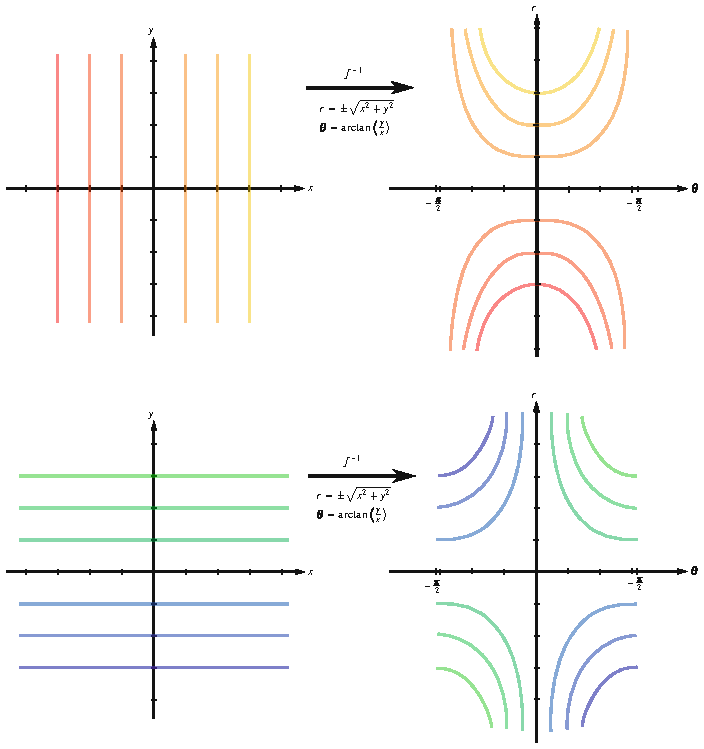
\includegraphics[width=0.960\linewidth]{images/vector/fig-6-9.pdf}
  \caption{极坐标变换 $f^{-1}:\mathbb{R}^2_{xy}\to\mathbb{R}^2_{r\theta}$ 被限制在 $-\pi/2<\theta\leq\pi/2$ 上. 这一限制是使 $f^{-1}$ 成为一一映射所必需的. 顶部显示了若干竖直直线的像，底部显示了若干水平直线的像}
  \label{fig:6-9}
\end{figure}

\begin{question}\label{q:6-6}
证明 $f^{-1}(x,y)$ 确实由 $f^{-1}(x,y)=\left(\pm\sqrt{x^2+y^2},\arctan\frac{y}{x}\right)$ 给出，其中当 $x\geq0$ 时取 $+$，当 $x<0$ 时取 $-$，且 $\theta$ 被限制在 $-\frac{\pi}{2}<\theta<\frac{\pi}{2}$.
\end{question}

\begin{question}\label{q:6-7}
类似于图~\ref{fig:6-9}，画出映射 $f:\mathbb{R}^2_{r\theta}\to\mathbb{R}^2_{xy}$ 的草图. 直线 $r=c$（$c$ 是常数）映射到哪里？直线 $\theta=c$ 映射到哪里？把这一点与你在微积分课上学到的极坐标知识进行比较.
\end{question}

实际上，要看出图~\ref{fig:6-9} 中 $\mathbb{R}^2_{xy}$ 上的水平直线和竖直直线映射到 $\mathbb{R}^2_{r\theta}$ 中的什么地方是相当容易的，我们只需把方程 $x=c$ 与 $y=c$（其中 $c$ 是常数）写成极坐标形式：
\[
x=c\ \Rightarrow\ c=r\cos\theta\ \Rightarrow\ r=\frac{c}{\cos\theta}=c\sec\theta
\]
而直线 $y=c$ 可以写成
\[
y=c\ \Rightarrow\ c=r\sin\theta\ \Rightarrow\ r=\frac{c}{\sin\theta}=c\csc\theta,
\]
其中 $-\frac{\pi}{2}<\theta<\frac{\pi}{2}$. 例如，直线 $x=1$ 可以写成 $r=\sec\theta$，直线 $x=2$ 写成 $r=2\sec\theta$，等等.

我们要在极坐标下做的第一件事是"把面积形式 $dx\wedge dy$ 写成 $d\theta\wedge dr$ 的形式". 利用映射 $f(r,\theta)=\bigl(x(r,\theta),y(r,\theta)\bigr)=\bigl(r\cos\theta,r\sin\theta\bigr)$ 求 $dx$ 和 $dy$：
\begin{align*}
dx&=\frac{\partial x}{\partial r}dr+\frac{\partial x}{\partial\theta}d\theta\\
&=\frac{\partial(r\cos\theta)}{\partial r}dr+\frac{\partial(r\cos\theta)}{\partial\theta}d\theta\\
&=\cos\theta\,dr-r\sin\theta\,d\theta
\end{align*}
以及
\begin{align*}
dy&=\frac{\partial y}{\partial r}dr+\frac{\partial y}{\partial\theta}d\theta\\
&=\frac{\partial(r\sin\theta)}{\partial r}dr+\frac{\partial(r\sin\theta)}{\partial\theta}d\theta\\
&=\sin\theta\,dr+r\cos\theta\,d\theta
\end{align*}
所以
\begin{align*}
dx\wedge dy&=\bigl(\cos\theta\,dr-r\sin\theta\,d\theta\bigr)\wedge\bigl(\sin\theta\,dr+r\cos\theta\,d\theta\bigr)\\
&=\cos\theta\sin\theta\underbrace{dr\wedge dr}_{=0}-r\sin^2\theta\,d\theta\wedge dr
+r\cos^2\theta\underbrace{dr\wedge d\theta}_{-d\theta\wedge dr}-r^2\sin\theta\cos\theta\underbrace{d\theta\wedge d\theta}_{=0}\\
&=-r(\sin^2\theta+\cos^2\theta)d\theta\wedge dr\\
&=-r\,d\theta\wedge dr.
\end{align*}
于是我们得到"恒等式" $dx\wedge dy=-r\,d\theta\wedge dr$. 既然我们已经"把面积形式 $dx\wedge dy$ 写成 $d\theta\wedge dr$ 的形式"，让我们分析一下我们实际上做了什么. 我们给定了一个映射 $f:\mathbb{R}^2_{r\theta}\to\mathbb{R}^2_{xy}$，我们学到了它诱导出如下作用的映射 $Tf$ 与 $T^*f$：
\[
\begin{gathered}
\bigwedge^2\mathbb{R}^2_{r\theta}\xleftarrow{T^*f}\bigwedge^2\mathbb{R}^2_{xy}\\
T^*f\cdot dx\wedge dy\longleftarrow dx\wedge dy\\
T\mathbb{R}^2_{r\theta}\xrightarrow{Tf}T\mathbb{R}^2_{xy}\\
\mathbb{R}^2_{r\theta}\xrightarrow{f}\mathbb{R}^2_{xy}.
\end{gathered}
\]
诱导映射 $T^*f$ 求 $\mathbb{R}^2_{xy}$ 上的体积形式被 $f$ 拉回的结果. 因此，当我们说我们已经"把面积形式 $dx\wedge dy$ 写成 $d\theta\wedge dr$ 的形式"时，我们实际上所做的是求拉回. 所以，恒等式 $dx\wedge dy=-r\,d\theta\wedge dr$ 实际上应该写成
\[
T^*f\cdot\bigl(dx\wedge dy\bigr)=-r\,d\theta\wedge dr.
\]

\begin{figure}[htbp]
  \centering
  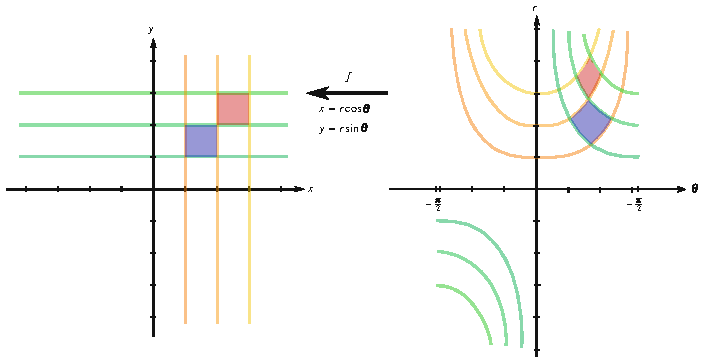
\includegraphics[width=0.960\linewidth]{images/vector/fig-6-10.pdf}
  \caption{映射 $f:\mathbb{R}^2_{r\theta}\to\mathbb{R}^2_{xy}$. 注意阴影区域发生了什么}
  \label{fig:6-10}
\end{figure}

\begin{question}\label{q:6-8}
参考图~\ref{fig:6-10}，用阴影区域解释公式 $T^*f\cdot\bigl(dx\wedge dy\bigr)=-r\,d\theta\wedge dr$.
\end{question}

类似地，我们可以用另一个方向的逆变换
\[
f^{-1}(x,y)=\bigl(r(x,y),\theta(x,y)\bigr)=\left(\pm\sqrt{x^2+y^2},\arctan\frac{y}{x}\right)
\]
来"把面积形式 $d\theta\wedge dr$ 写成 $dx\wedge dy$ 的形式". 首先我们需要求 $d\theta$ 与 $dr$：
\begin{align*}
d\theta&=\frac{\partial\theta}{\partial x}dx+\frac{\partial\theta}{\partial y}dy\\
&=\frac{\partial\arctan(y/x)}{\partial x}dx+\frac{\partial\arctan(y/x)}{\partial y}dy\\
&\overset{\text{链式法则}}{=}\frac{1}{1+(y/x)^2}\frac{\partial}{\partial x}\left(\frac{y}{x}\right)dx
+\frac{1}{1+(y/x)^2}\frac{\partial}{\partial y}\left(\frac{y}{x}\right)dy\\
&=\frac{-y}{x^2+y^2}dx+\frac{x}{x^2+y^2}dy
\end{align*}
以及
\begin{align*}
dr&=\frac{\partial r}{\partial x}dx+\frac{\partial r}{\partial y}dy\\
&=\frac{\partial\bigl(\pm\sqrt{x^2+y^2}\bigr)}{\partial x}dx+\frac{\partial\bigl(\pm\sqrt{x^2+y^2}\bigr)}{\partial y}dy\\
&\overset{\text{链式法则}}{=}\pm\frac{x}{\sqrt{x^2+y^2}}dx\pm\frac{y}{\sqrt{x^2+y^2}}dy
\end{align*}
所以
\begin{align*}
d\theta\wedge dr
&=\left(\frac{-y}{x^2+y^2}dx+\frac{x}{x^2+y^2}dy\right)
\wedge\left(\pm\frac{x}{\sqrt{x^2+y^2}}dx\pm\frac{y}{\sqrt{x^2+y^2}}dy\right)\\
&=\pm\frac{x^2}{(x^2+y^2)\sqrt{x^2+y^2}}dy\wedge dx
-\pm\frac{y^2}{(x^2+y^2)\sqrt{x^2+y^2}}dx\wedge dy\\
&=\pm\frac{-(x^2+y^2)}{(x^2+y^2)\sqrt{x^2+y^2}}dx\wedge dy\\
&=\pm\frac{-1}{\sqrt{x^2+y^2}}dx\wedge dy.
\end{align*}
于是我们得到了恒等式 $d\theta\wedge dr=\frac{-1}{\sqrt{x^2+y^2}}dx\wedge dy$. 和之前一样，我们给定了一个映射 $f^{-1}:\mathbb{R}^2_{xy}\to\mathbb{R}^2_{r\theta}$，它诱导出映射 $Tf^{-1}$ 与 $T^*f^{-1}$，使得
\[
\begin{gathered}
\bigwedge^2\mathbb{R}^2_{xy}\xleftarrow{T^*f^{-1}}\bigwedge^2\mathbb{R}^2_{r\theta}\\
T^*f^{-1}\cdot d\theta\wedge dr\longleftarrow d\theta\wedge dr\\
T\mathbb{R}^2_{xy}\xrightarrow{Tf^{-1}}T\mathbb{R}^2_{r\theta}\\
\mathbb{R}^2_{xy}\xrightarrow{f^{-1}}\mathbb{R}^2_{r\theta}.
\end{gathered}
\]
所以当我们说"把面积形式 $d\theta\wedge dr$ 写成 $dx\wedge dy$ 的形式"时，我们真正的意思是求拉回. 我们得到的恒等式 $d\theta\wedge dr=\frac{-1}{\sqrt{x^2+y^2}}dx\wedge dy$ 实际上应该写成
\[
T^*f^{-1}\cdot\bigl(d\theta\wedge dr\bigr)=\pm\frac{-1}{\sqrt{x^2+y^2}}dx\wedge dy.
\]
由于我们这里实际上处理的是体积形式，我们本可以用另一种方法做所有这些，即利用上一节导出的体积形式拉回的一般公式. 也就是说，给定映射 $\phi:\mathbb{R}^n\to\mathbb{R}^n$，其中
\[
\phi=\bigl(\phi_1(x_1,\ldots,x_n),\phi_2(x_1,\ldots,x_n),\ldots,\phi_n(x_1,\ldots,x_n)\bigr),
\]
体积形式的拉回由下面的等式给出
\[
T^*\phi\cdot\bigl(d\phi_1\wedge d\phi_2\wedge\cdots\wedge d\phi_n\bigr)
=\left|\begin{matrix}
\frac{\partial\phi_1}{\partial x_1}&\frac{\partial\phi_1}{\partial x_2}&\cdots&\frac{\partial\phi_1}{\partial x_n}\\
\frac{\partial\phi_2}{\partial x_1}&\frac{\partial\phi_2}{\partial x_2}&\cdots&\frac{\partial\phi_2}{\partial x_n}\\
\vdots&\vdots&\ddots&\vdots\\
\frac{\partial\phi_n}{\partial x_1}&\frac{\partial\phi_n}{\partial x_2}&\cdots&\frac{\partial\phi_n}{\partial x_n}
\end{matrix}\right|dx_1\wedge dx_2\wedge\cdots\wedge dx_n.
\]
回想一下，体积形式是特殊的. 虽然 Jacobian 矩阵总是给出 $T\phi$，因此总是被用来求向量的前推，但 Jacobian 矩阵只能用来求体积形式的拉回，而不能用来求不是体积形式的其他微分形式的拉回.

首先我们求映射 $f^{-1}(x,y)=\left(\arctan\frac{y}{x},\pm\sqrt{x^2+y^2}\right)$ 的 Jacobian 矩阵为
\[
\begin{bmatrix}
\frac{\partial\theta}{\partial x}&\frac{\partial\theta}{\partial y}\\
\frac{\partial r}{\partial x}&\frac{\partial r}{\partial y}
\end{bmatrix}
=
\begin{bmatrix}
\frac{-y}{x^2+y^2}&\frac{x}{x^2+y^2}\\
\pm\frac{x}{\sqrt{x^2+y^2}}&\pm\frac{y}{\sqrt{x^2+y^2}}
\end{bmatrix}
\]
其行列式为
\[
\left|\begin{matrix}
\frac{-y}{x^2+y^2}&\frac{x}{x^2+y^2}\\
\pm\frac{x}{\sqrt{x^2+y^2}}&\pm\frac{y}{\sqrt{x^2+y^2}}
\end{matrix}\right|
=\pm\frac{-y^2-x^2}{(x^2+y^2)\sqrt{x^2+y^2}}
=\pm\frac{-1}{\sqrt{x^2+y^2}}
\]
这直接给出
\[
T^*f^{-1}\cdot\bigl(d\theta\wedge dr\bigr)=\pm\frac{-1}{\sqrt{x^2+y^2}}dx\wedge dy.
\]
另一个方向也类似地完成：
\[
\left|\begin{matrix}
\frac{\partial x}{\partial\theta}&\frac{\partial x}{\partial r}\\
\frac{\partial y}{\partial\theta}&\frac{\partial y}{\partial r}
\end{matrix}\right|
=
\left|\begin{matrix}
-r\sin\theta&\cos\theta\\
r\cos\theta&\sin\theta
\end{matrix}\right|
=-r\sin^2\theta-r\cos^2\theta=-r
\]
这给出
\[
T^*f\cdot\bigl(dx\wedge dy\bigr)=-r\,d\theta\wedge dr.
\]

现在我们为一个极坐标的例子逐步演算. 通过这个例子和下面的问题，我们将探索笛卡尔坐标与极坐标之间的变换与我们前面几节考察的线性例子相当不同的方式之一. 极坐标变换与线性坐标变换不同的地方在于：两个体积形式之间的关系取决于我们在哪个点. 也就是说，拉回方程取决于基点.

对于由 $f^{-1}(x,y)=\left(\arctan\frac{y}{x},\pm\sqrt{x^2+y^2}\right)$ 给出的极坐标变换 $f^{-1}:\mathbb{R}^2_{xy}\to\mathbb{R}^2_{r\theta}$，我们以弧度给出 $\theta$. 我们的目标是把
\[
(dx\wedge dy)_{(1,1)}\left(\binom{1}{0}_{(1,1)},\binom{0}{1}_{(1,1)}\right)
\]
与
\[
(d\theta\wedge dr)_{f^{-1}(1,1)}\left(T_{(1,1)}f^{-1}\cdot\binom{1}{0}_{(1,1)},T_{(1,1)}f^{-1}\cdot\binom{0}{1}_{(1,1)}\right)
\]
联系起来. 第一个恒等式很简单，我们得到
\[
(dx\wedge dy)_{(1,1)}\left(\binom{1}{0}_{(1,1)},\binom{0}{1}_{(1,1)}\right)
=\left|\begin{matrix}1&0\\0&1\end{matrix}\right|=1.
\]
这里我们用 $xy$ 平面体积形式 $dx\wedge dy$ 求由两个欧几里得单位向量张成的平行六面体的面积. 不出所料，我们得到体积 $1$，正是我们对单位正方形的预期. 现在我们转到下一个恒等式. 首先我们求出 $f^{-1}(1,1)\approx(0.785,1.414)$. 这就是两个欧几里得单位向量的前推的基点. 接下来我们求一般的切映射
\[
T_{(x,y)}f^{-1}
=
\begin{bmatrix}
\frac{\partial\theta}{\partial x}&\frac{\partial\theta}{\partial y}\\
\frac{\partial r}{\partial x}&\frac{\partial r}{\partial y}
\end{bmatrix}
=
\begin{bmatrix}
\frac{-y}{x^2+y^2}&\frac{x}{x^2+y^2}\\
\pm\frac{x}{\sqrt{x^2+y^2}}&\pm\frac{y}{\sqrt{x^2+y^2}}
\end{bmatrix}_{(x,y)}
\]
这意味着对点 $(x,y)=(1,1)$ 我们有
\[
T_{(1,1)}f^{-1}=
\begin{bmatrix}
-\frac12&\frac12\\
\frac{1}{\sqrt{2}}&\frac{1}{\sqrt{2}}
\end{bmatrix}_{(1,1)}.
\]

\begin{figure}[htbp]
  \centering
  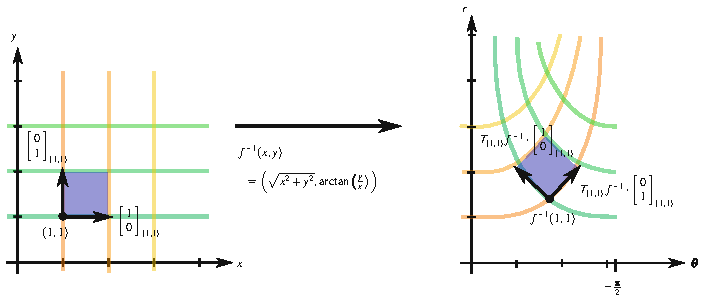
\includegraphics[width=0.960\linewidth]{images/vector/fig-6-11.pdf}
  \caption{在点 $(x,y)=(1,1)$ 与 $f^{-1}(1,1)$ 处体积形式 $dx\wedge dy$ 与 $d\theta\wedge dr$ 之间的关系}
  \label{fig:6-11}
\end{figure}

接下来我们求欧几里得单位向量在 $(1,1)$ 处被 $f^{-1}$ 的前推：
\begin{align*}
T_{(1,1)}f^{-1}\cdot\binom{1}{0}_{(1,1)}
=
\begin{bmatrix}
-\frac12&\frac12\\
\frac{1}{\sqrt{2}}&\frac{1}{\sqrt{2}}
\end{bmatrix}_{(1,1)}
\cdot\binom{1}{0}_{(1,1)}
=
\begin{bmatrix}
-\frac12\\
\frac{1}{\sqrt{2}}
\end{bmatrix}_{(0.785,1.414)}, \\
T_{(1,1)}f^{-1}\cdot\binom{0}{1}_{(1,1)}
=
\begin{bmatrix}
-\frac12&\frac12\\
\frac{1}{\sqrt{2}}&\frac{1}{\sqrt{2}}
\end{bmatrix}_{(1,1)}
\cdot\binom{0}{1}_{(1,1)}
=
\begin{bmatrix}
\frac12\\
\frac{1}{\sqrt{2}}
\end{bmatrix}_{(0.785,1.414)},
\end{align*}
它们被用在
\[
(d\theta\wedge dr)_{(0.785,1.414)}\left(
\begin{bmatrix}
-\frac12\\
\frac{1}{\sqrt{2}}
\end{bmatrix}_{(0.785,1.414)},
\begin{bmatrix}
\frac12\\
\frac{1}{\sqrt{2}}
\end{bmatrix}_{(0.785,1.414)}
\right)
=\left|\begin{matrix}-\frac12&\frac12\\\frac{1}{\sqrt{2}}&\frac{1}{\sqrt{2}}\end{matrix}\right|
=\frac{-1}{\sqrt{2}}.
\]
这里我们用 $r\theta$ 平面体积形式求由被前推的向量张成的平行六面体的体积. 以这种方式算出的面积之间的关系，与在点 $(1,1)\in\mathbb{R}^2_{xy}$ 处由 $T^*f^{-1}\cdot\bigl(d\theta\wedge dr\bigr)=\frac{-1}{\sqrt{x^2+y^2}}dx\wedge dy$ 给出的体积形式 $dx\wedge dy$ 与 $d\theta\wedge dr$ 之间的关系精确对应. 也就是说，
\[
\begin{aligned}
(d\theta\wedge dr)_{f^{-1}(1,1)}&\left(T_{(1,1)}f^{-1}\cdot\binom{1}{0}_{(1,1)},T_{(1,1)}f^{-1}\cdot\binom{0}{1}_{(1,1)}\right)\\
&=\frac{-1}{\sqrt{2}}(dx\wedge dy)_{(1,1)}\left(\binom{1}{0}_{(1,1)},\binom{0}{1}_{(1,1)}\right).
\end{aligned}
\]
换句话说，我们刚刚看到，利用在点 $(1,1)$ 处的两个向量，有
\[
T^*f^{-1}(d\theta\wedge dr)=\frac{-1}{\sqrt{2}}dx\wedge dy.
\]
我们试图在图~\ref{fig:6-11} 中展示正在发生的事情. 现在换一个不同的基点重做最后一个例子，看看会发生什么变化.

\begin{question}\label{q:6-9}
对于由 $f^{-1}(x,y)=\left(\arctan\frac{y}{x},\pm\sqrt{x^2+y^2}\right)$ 给出的极坐标变换 $f^{-1}:\mathbb{R}^2_{xy}\to\mathbb{R}^2_{r\theta}$：
\begin{enumerate}
  \item[(a)] 求 $f^{-1}(2,2)$.
  \item[(b)] 考虑 $\binom{1}{0}_{(2,2)}$ 与 $\binom{0}{1}_{(2,2)}\in T_{(2,2)}\mathbb{R}^2$. 求 $(dx\wedge dy)_{(2,2)}\left(\binom{1}{0}_{(2,2)},\binom{0}{1}_{(2,2)}\right)$.
  \item[(c)] 求 $T_{(2,2)}f^{-1}$.
  \item[(d)] 求 $T_{(2,2)}f^{-1}\cdot\binom{1}{0}_{(2,2)}$ 与 $T_{(2,2)}f^{-1}\cdot\binom{0}{1}_{(2,2)}$. （这些是欧几里得单位向量在 $(2,2)$ 处被 $f^{-1}$ 前推到 $f^{-1}(2,2)$ 的结果.）
  \item[(e)] 求 $(d\theta\wedge dr)_{f^{-1}(2,2)}\left(T_{(2,2)}f^{-1}\cdot\binom{1}{0}_{(2,2)},T_{(2,2)}f^{-1}\cdot\binom{0}{1}_{(2,2)}\right)$.
\end{enumerate}
\end{question}

图~\ref{fig:6-12} 展示了这道题中发生的事情. 你在这道题中应该得到的关系是
\[
\begin{aligned}
(d\theta\wedge dr)_{f^{-1}(2,2)}&\left(T_{(2,2)}f^{-1}\cdot\binom{1}{0}_{(2,2)},T_{(2,2)}f^{-1}\cdot\binom{0}{1}_{(2,2)}\right)\\
&=\frac{-1}{\sqrt{8}}(dx\wedge dy)_{(2,2)}\left(\binom{1}{0}_{(2,2)},\binom{0}{1}_{(2,2)}\right).
\end{aligned}
\]
数值系数发生了变化. 这是因为我们求面积的基点发生了变化. 换句话说，$xy$ 平面与 $r\theta$ 平面中面积形式之间的关系取决于面积形式被使用的点. 所以，在点 $(1,1)$ 处我们有
\[
T_{(1,1)}^*f^{-1}\cdot\bigl(d\theta\wedge dr\bigr)=\frac{-1}{\sqrt{2}}dx\wedge dy
\]
而在点 $(2,2)$ 处我们有
\[
T_{(2,2)}^*f^{-1}\cdot\bigl(d\theta\wedge dr\bigr)=\frac{-1}{\sqrt{8}}dx\wedge dy
\]
这正是我们从前面的实际恒等式所预期的：
\[
T_{(x,y)}^*f^{-1}\cdot\bigl(d\theta\wedge dr\bigr)=\pm\frac{-1}{\sqrt{x^2+y^2}}dx\wedge dy.
\]

\begin{figure}[htbp]
  \centering
  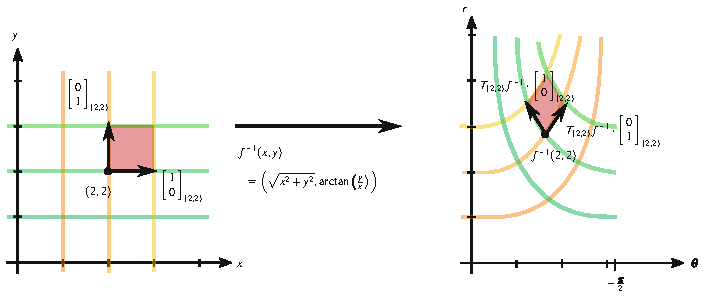
\includegraphics[width=0.960\linewidth]{images/vector/fig-6-12.pdf}
  \caption{在点 $(x,y)=(2,2)$ 与 $f^{-1}(2,2)$ 处体积形式 $dx\wedge dy$ 与 $d\theta\wedge dr$ 之间的关系}
  \label{fig:6-12}
\end{figure}

\section{柱坐标与球坐标}

柱坐标与球坐标是 $\mathbb{R}^3$ 非常常用的两个坐标系. 既然我们现在对向量的前推与体积形式的拉回有了相当好的认识，我们将在本节提供较少的细节. 柱坐标变换 $f:\mathbb{R}^3_{r\theta z}\to\mathbb{R}^3_{xyz}$ 由
\[
f(r,\theta,z)=\bigl(x(r,\theta,z),y(r,\theta,z),z(r,\theta,z)\bigr)=\bigl(r\cos\theta,r\sin\theta,z\bigr)
\]
给出，在微积分课上它一般写成
\[
x=r\cos\theta,\qquad y=r\sin\theta,\qquad z=z.
\]
见图~\ref{fig:6-13}. 柱坐标变换 $f$ 诱导出如下映射：
\[
\begin{gathered}
\bigwedge^3\mathbb{R}^3_{r\theta z}\xleftarrow{T^*f}\bigwedge^3\mathbb{R}^3_{xyz}\\
T_{(r,\theta,z)}^*f\cdot\bigl(dx\wedge dy\wedge dz\bigr)\longleftarrow dx\wedge dy\wedge dz\\
\mathbb{R}^3_{r\theta z}\xrightarrow{Tf}\mathbb{R}^3_{xyz}\\
v_{(r,\theta,z)}\longmapsto T_{(r,\theta,z)}f\cdot v_{(r,\theta,z)}\\
\mathbb{R}^3_{r\theta z}\xrightarrow{f}\mathbb{R}^3_{xyz}\\
(r,\theta,z)\longmapsto\bigl(r\cos\theta,r\sin\theta,z\bigr).
\end{gathered}
\]

\begin{figure}[htbp]
  \centering
  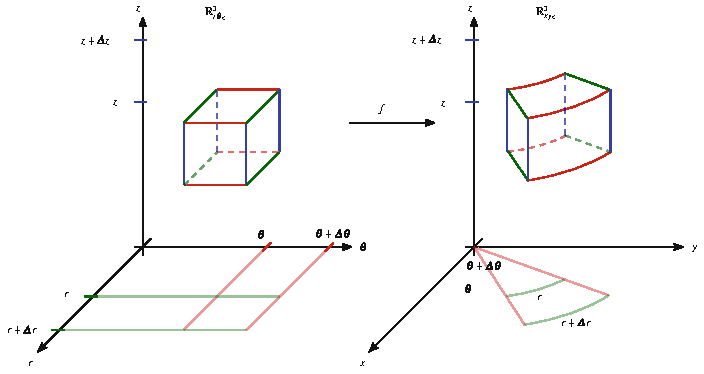
\includegraphics[width=0.960\linewidth]{images/vector/fig-6-13.pdf}
  \caption{由 $x=r\cos\theta$、$y=r\sin\theta$、$z=z$ 给出的柱坐标映射 $f:\mathbb{R}^3_{r\theta z}\to\mathbb{R}^3_{xyz}$. $\mathbb{R}^3_{r\theta z}$ 中的立方体被映射为 $\mathbb{R}^3_{xyz}$ 中的楔形体}
  \label{fig:6-13}
\end{figure}

和之前一样进行，要么利用楔积的性质，要么利用以 Jacobian 形式给出的楔积公式，我们可以把 $dx\wedge dy\wedge dz$ 写成 $d\theta\wedge dr\wedge dz$ 的形式. 这里我们求
\begin{align*}
dx=\frac{\partial x}{\partial\theta}d\theta+\frac{\partial x}{\partial r}dr+\frac{\partial x}{\partial z}dz=-r\sin\theta\,d\theta+\cos\theta\,dr, \\
dy=\frac{\partial y}{\partial\theta}d\theta+\frac{\partial y}{\partial r}dr+\frac{\partial y}{\partial z}dz=r\cos\theta\,d\theta+\sin\theta\,dr, \\
dz=\frac{\partial z}{\partial\theta}d\theta+\frac{\partial z}{\partial r}dr+\frac{\partial z}{\partial z}dz=dz
\end{align*}
我们用它来得到
\begin{align*}
dx\wedge dy\wedge dz&=\bigl(-r\sin\theta\,d\theta+\cos\theta\,dr\bigr)\wedge\bigl(r\cos\theta\,d\theta+\sin\theta\,dr\bigr)\wedge dz\\
&=\bigl(-r\sin^2\theta\,d\theta\wedge dr+r\cos^2\theta\,dr\wedge d\theta\bigr)\wedge dz\\
&=-r\,d\theta\wedge dr\wedge dz.
\end{align*}
正如我们现在所知，这个恒等式的真正含义是
\[
T_{(r,\theta,z)}^*f\cdot\bigl(dx\wedge dy\wedge dz\bigr)=-r\,d\theta\wedge dr\wedge dz.
\]
我们刚才所做的正是求微积分中通常给出的"$\theta rz$ 体积元". 很多微积分书给出一个看起来像图~\ref{fig:6-14} 的"$\theta rz$ 体积元"图画，然后用这幅图来求体积变化公式，尽管定向没有被考虑进去. 因此，即使我们的处理方式比你见过的任何微积分都抽象和理论化得多，你对它也已经从另一个视角熟悉了.

\begin{figure}[htbp]
  \centering
  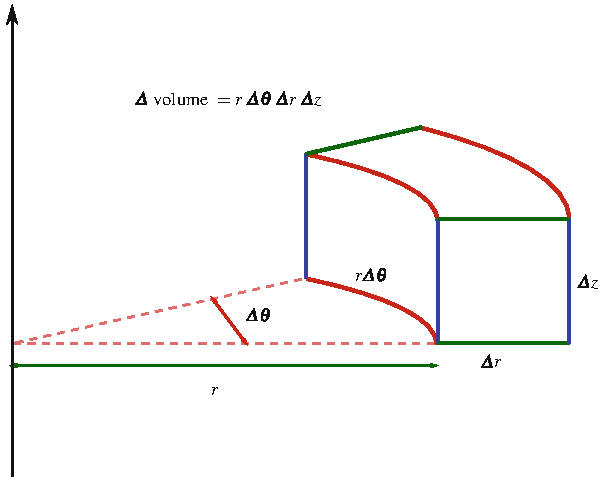
\includegraphics[width=0.717\linewidth]{images/vector/fig-6-14.pdf}
  \caption{大多数微积分教科书中给出的柱坐标"$\theta rz$ 体积元"}
  \label{fig:6-14}
\end{figure}

\begin{question}\label{q:6-10}
利用体积形式拉回的公式求 $T_{(r,\theta,z)}^*f\cdot\bigl(dx\wedge dy\wedge dz\bigr)$.
\end{question}

\begin{question}\label{q:6-11}
解释公式 $T_{(r,\theta,z)}^*f\cdot\bigl(dx\wedge dy\wedge dz\bigr)=-r\,d\theta\wedge dr\wedge dz$ 与图~\ref{fig:6-14} 所示"$\theta rz$ 体积元"之间的关系.
\end{question}

现在我们转向球坐标变换. 球坐标变换 $g:\mathbb{R}^3_{\rho\varphi\theta}\to\mathbb{R}^3_{xyz}$ 由
\[
g(\rho,\varphi,\theta)=\bigl(x(\rho,\varphi,\theta),y(\rho,\varphi,\theta),z(\rho,\varphi,\theta)\bigr)
=\bigl(\rho\sin\varphi\cos\theta,\rho\sin\varphi\sin\theta,\rho\cos\varphi\bigr)
\]
给出，在微积分课上它一般写成
\[
x=\rho\sin\varphi\cos\theta,\qquad y=\rho\sin\varphi\sin\theta,\qquad z=\rho\cos\varphi.
\]
映射 $g:\mathbb{R}^3_{\rho\varphi\theta}\to\mathbb{R}^3_{xyz}$ 在图~\ref{fig:6-15} 中作了说明. 球坐标变换诱导出如下映射：
\[
\begin{gathered}
\bigwedge^3\mathbb{R}^3_{\rho\varphi\theta}\xleftarrow{T^*g}\bigwedge^3\mathbb{R}^3_{xyz}\\
T_{(\rho,\varphi,\theta)}^*g\cdot\bigl(dx\wedge dy\wedge dz\bigr)\longleftarrow dx\wedge dy\wedge dz\\
\mathbb{R}^3_{\rho\varphi\theta}\xrightarrow{Tg}\mathbb{R}^3_{xyz}\\
v_{(\rho,\varphi,\theta)}\longmapsto T_{(\rho,\varphi,\theta)}g\cdot v_{(\rho,\varphi,\theta)}\\
\mathbb{R}^3_{\rho\varphi\theta}\xrightarrow{g}\mathbb{R}^3_{xyz}\\
(\rho,\varphi,\theta)\longmapsto\bigl(\rho\sin\varphi\cos\theta,\rho\sin\varphi\sin\theta,\rho\cos\varphi\bigr).
\end{gathered}
\]

\begin{figure}[htbp]
  \centering
  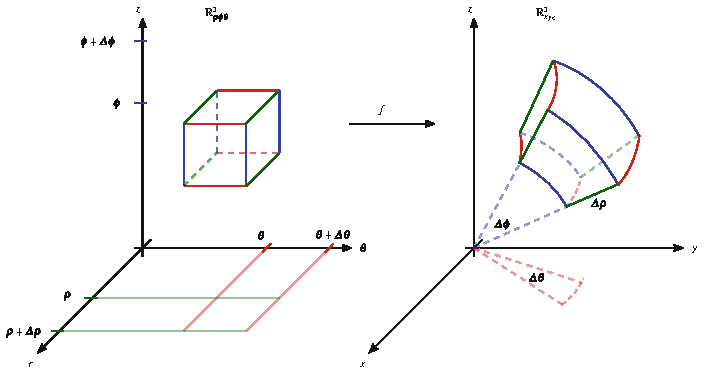
\includegraphics[width=0.960\linewidth]{images/vector/fig-6-15.pdf}
  \caption{由 $x=\rho\sin\varphi\cos\theta$、$y=\rho\sin\varphi\sin\theta$、$z=\rho\cos\varphi$ 给出的球坐标变换 $g:\mathbb{R}^3_{\rho\varphi\theta}\to\mathbb{R}^3_{xyz}$}
  \label{fig:6-15}
\end{figure}

同样，一个直截了当的计算表明
\begin{align*}
dx=\sin\varphi\cos\theta\,d\rho-\rho\sin\varphi\sin\theta\,d\theta+\rho\cos\varphi\cos\theta\,d\varphi, \\
dy=\sin\varphi\sin\theta\,d\rho+\rho\sin\varphi\cos\theta\,d\theta+\rho\cos\varphi\sin\theta\,d\varphi, \\
dz=\cos\varphi\,d\rho-\rho\sin\varphi\,d\varphi.
\end{align*}
另一个直截了当但稍长一些、应该由你自己完成的计算给出
\[
dx\wedge dy\wedge dz=-\rho^2\sin\varphi\,d\rho\wedge d\theta\wedge d\varphi.
\]
正如我们现在所知道的，这个恒等式的真正含义是
\[
T_{(\rho,\varphi,\theta)}^*g\cdot\bigl(dx\wedge dy\wedge dz\bigr)=-\rho^2\sin\varphi\,d\rho\wedge d\theta\wedge d\varphi.
\]
由于 $dx\wedge dy\wedge dz$ 是体积形式，我们本可以用体积形式拉回的公式求出它. 很多微积分书给出一个看起来像图~\ref{fig:6-16} 的"$\rho\varphi\theta$ 体积元"图画. 注意我们如何能从这幅图图解地看出体积的变化，尽管定向仍然没有被考虑进去. 所以同样，尽管我们从更抽象的角度来讨论这一点，但这是你在微积分中已经接触过的东西.

\begin{figure}[htbp]
  \centering
  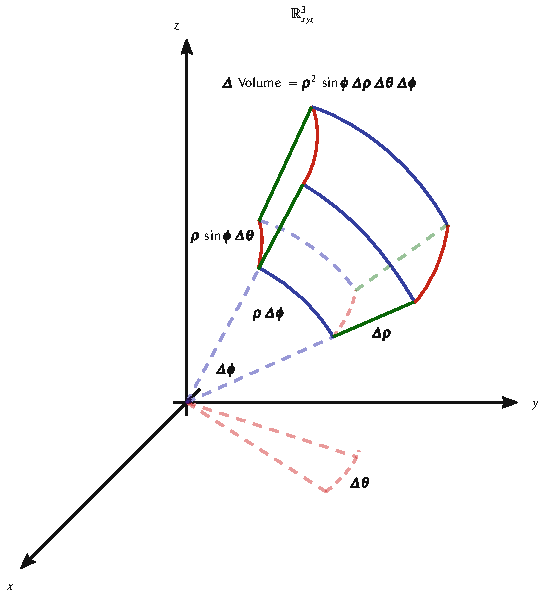
\includegraphics[width=0.715\linewidth]{images/vector/fig-6-16.pdf}
  \caption{大多数微积分教科书中给出的球坐标"$\rho\varphi\theta$ 体积元"}
  \label{fig:6-16}
\end{figure}

\begin{question}\label{q:6-12}
利用体积形式拉回的公式求 $T_{(\rho,\varphi,\theta)}^*g\cdot\bigl(dx\wedge dy\wedge dz\bigr)$.
\end{question}

\begin{question}\label{q:6-13}
解释公式 $T_{(\rho,\varphi,\theta)}^*g\cdot\bigl(dx\wedge dy\wedge dz\bigr)=-\rho^2\sin\varphi\,d\rho\wedge d\theta\wedge d\varphi$ 与图~\ref{fig:6-16} 所示"$\rho\varphi\theta$ 体积元"之间的关系.
\end{question}

\section{微分形式的拉回}

考虑我们在前几节得到的若干关系
\begin{align*}
T^*f\cdot(dx\wedge dy)=-\frac12du\wedge dv\qquad\text{(线性例子)} \\
T^*f\cdot(dx\wedge dy)=-r\,d\theta\wedge dr\qquad\text{(极坐标)} \\
T^*f\cdot(dx\wedge dy\wedge dz)=-r\,d\theta\wedge dr\wedge dz\qquad\text{(柱坐标)} \\
T^*f\cdot(dx\wedge dy\wedge dz)=-\rho^2\sin\varphi\,d\rho\wedge d\theta\wedge d\varphi\qquad\text{(球坐标)}
\end{align*}
其中 $f$ 是相应的映射 $f:\mathbb{R}^{n}_{\text{其他坐标}}\to\mathbb{R}^{n}_{\text{欧几里得}}$. 根据我们给出的体积形式拉回的定义，这些式子真正意味着
\begin{align*}
\underbrace{-\frac12(du\wedge dv)_p(v_p,w_p)}_{=\ T_p^*f\cdot(dx\wedge dy)_{f(p)}}=(dx\wedge dy)_{f(p)}(T_pf\cdot v_p,T_pf\cdot w_p), \\
\underbrace{-r(d\theta\wedge dr)_p(v_p,w_p)}_{=\ T_p^*f\cdot(dx\wedge dy)_{f(p)}}=(dx\wedge dy)_{f(p)}(T_pf\cdot v_p,T_pf\cdot w_p), \\
\underbrace{-r(d\theta\wedge dr\wedge dz)_p(u_p,v_p,w_p)}_{=\ T_p^*f\cdot(dx\wedge dy\wedge dz)_{f(p)}}=(dx\wedge dy\wedge dz)_{f(p)}(T_pf\cdot u_p,T_pf\cdot v_p,T_pf\cdot w_p), \\
\underbrace{-\rho^2\sin\varphi(d\rho\wedge d\theta\wedge d\varphi)_p(u_p,v_p,w_p)}_{=\ T_p^*f\cdot(dx\wedge dy\wedge dz)_{f(p)}}=(dx\wedge dy\wedge dz)_{f(p)}(T_pf\cdot u_p,T_pf\cdot v_p,T_pf\cdot w_p).
\end{align*}

现在我们花一点时间再详细地给出微分形式拉回的定义. 假设我们有映射 $\varphi:\mathbb{R}^n\to\mathbb{R}^m$，其中
\[
\varphi(x_1,x_2,\ldots,x_n)=\bigl(\varphi_1(x_1,x_2,\ldots,x_n),\varphi_2(x_1,x_2,\ldots,x_n),\ldots,\varphi_m(x_1,x_2,\ldots,x_n)\bigr).
\]
$\varphi$ 定义一个映射，称为 $\varphi$ 的前推或切映射，记为 $T\varphi:T\mathbb{R}^n\to T\mathbb{R}^m$，它从 $\mathbb{R}^n$ 的切丛到 $\mathbb{R}^m$ 的切丛. 在坐标下，映射 $T\varphi$ 由 Jacobian 矩阵给出：
\[
T\varphi=
\begin{bmatrix}
\frac{\partial\varphi_1}{\partial x_1}&\cdots&\frac{\partial\varphi_1}{\partial x_n}\\
\vdots&\ddots&\vdots\\
\frac{\partial\varphi_m}{\partial x_1}&\cdots&\frac{\partial\varphi_m}{\partial x_n}
\end{bmatrix}.
\]
正如已经提到过的，人们经常遇到的 $T\varphi$ 的其他记号是 $D\varphi$ 与 $\varphi_*$. 我们用这个前推映射 $T\varphi$ 来帮助定义另一个映射，称为微分形式被 $\varphi$ 的拉回，或简称为被 $\varphi$ 的拉回，记为 $T^*\varphi$ 或 $\varphi^*$. 实际上，$\varphi^*$ 是拉回的标准记号，但我们将使用 $T^*\varphi$.

在真正定义 $T^*\varphi$ 之前，我们要说明它作用于哪些空间. 回想记号 $\bigwedge^k\mathbb{R}^n$ 用来表示 $\mathbb{R}^n$ 上 $k$-形式的向量空间，而
\[
\bigwedge\mathbb{R}^n=\bigcup_{k=1}^{\infty}\bigwedge^k\mathbb{R}^n
\]
表示 $\mathbb{R}^n$ 上任意大小的所有微分形式的集合. 利用这一点，我们一般把映射 $\varphi$ 及其诱导映射 $T\varphi$ 与 $T^*\varphi$ 画成
\[
\begin{gathered}
\bigwedge\mathbb{R}^n\xleftarrow{T^*\varphi}\bigwedge\mathbb{R}^m\\
T\mathbb{R}^n\xrightarrow{T\varphi}T\mathbb{R}^m\\
\mathbb{R}^n\xrightarrow{\varphi}\mathbb{R}^m.
\end{gathered}
\]
所以，拉回映射作用于空间 $\bigwedge\mathbb{R}^m$，它取 $\mathbb{R}^m$ 上的一个微分形式，产生 $\bigwedge\mathbb{R}^n$ 的一个元素，即 $\mathbb{R}^n$ 上的一个微分形式. 注意这个映射的方向与 $\varphi$ 和 $T\varphi$ 相反. 这就是为什么 $T^*\varphi$ 被称为拉回而 $T\varphi$ 被称为前推. 接下来，即使 $T^*\varphi$ 作用于任意阶的 $k$-形式，我们有时也滥用记号写成
\[
T^*\mathbb{R}^n\xleftarrow{T^*\varphi}T^*\mathbb{R}^m,
\]
即用 $T^*\mathbb{R}^n$ 与 $T^*\mathbb{R}^m$ 代替 $\bigwedge\mathbb{R}^n$ 与 $\bigwedge\mathbb{R}^m$. 我们把 $k$-形式 $\alpha$ 的拉回，即 $T^*\varphi\cdot\alpha\in\bigwedge^k\mathbb{R}^n$，定义为 $\alpha\in\bigwedge^k\mathbb{R}^m$ 作用于被前推的向量 $T\varphi\cdot v_i\in T\mathbb{R}^m$：

\begin{definition}[$\alpha$ 的拉回]\label{def:6-6-1}
\[
\bigl(T^*\varphi\cdot\alpha\bigr)(v_1,v_2,\ldots,v_k)\equiv\alpha\bigl(T\varphi\cdot v_1,T\varphi\cdot v_2,\ldots,T\varphi\cdot v_k\bigr).
\]
\end{definition}

如果我们想小心一点并开始跟踪基点，记号就开始变得有点笨拙了，尽管有时你确实需要这样做. 这个记号的一个奇怪之处是，映射 $T^*\varphi$ 不是按它来自的点加下标，而是按它去往的点加下标. 这样做是为了使拉回与前推映射 $T_p^*\varphi$ 与 $T_p\varphi$ 的记号保持一致，也就是说，使它们彼此"对偶". 这种事情并不常发生，而且你头几次看到它时肯定会觉得奇怪.
\[
\begin{gathered}
\mathbb{R}^n_p\xleftarrow{T_p^*\varphi}\mathbb{R}^m_{\varphi(p)}\\
T_p\mathbb{R}^n\xrightarrow{T_p\varphi}T_{\varphi(p)}\mathbb{R}^m\\
\mathbb{R}^n\xrightarrow{\varphi}\mathbb{R}^m.
\end{gathered}
\]
加上基点之后，我们有以下定义
\[
\underbrace{\bigl(T_p^*\varphi\cdot\alpha_{\varphi(p)}\bigr)\bigl(v_{1_p},v_{2_p},\ldots,v_{k_p}\bigr)}_{\text{$\alpha$ 的拉回}}\equiv\alpha_{\varphi(p)}\bigl(T_p\varphi\cdot v_{1_p},T_p\varphi\cdot v_{2_p},\ldots,T_p\varphi\cdot v_{k_p}\bigr).
\]

现在，为了实际看到这是如何工作的，让我们考虑几个例子. 我们已经大量研究了体积形式，所以现在我们转向任意 $k$ 的 $k$-形式. 遗憾的是没有求任意形式拉回的好公式，但有一个相当标准的步骤可以使用. 考虑由 $\varphi(x,y)=(x+y,x-y)$ 给出的映射 $\varphi:\mathbb{R}^2_{xy}\to\mathbb{R}^2_{uv}$ 以及 $\mathbb{R}^2_{uv}$ 上的 1-形式 $\alpha=vdu+udv$. 我们想在 $\mathbb{R}^2_{xy}$ 上求 $T^*\varphi\cdot\alpha$. 注意，我们现在处理的是一个 1-形式，而不是体积形式.

我们将按如下方式处理这个问题. $\alpha$ 的拉回 $T^*\varphi\cdot\alpha$ 将是 $\mathbb{R}^2_{xy}$ 上的一个 1-形式，因此它将具有 $f(x,y)dx+g(x,y)dy$ 的形式，其中 $f$ 与 $g$ 是迄今未知的函数. 正是这些函数是我们想求的. 首先我们注意到
\[
(fdx+gdy)\binom{1}{0}=f\,dx\binom{1}{0}+g\,dy\binom{1}{0}=f(1)+g(0)=f
\]
以及
\[
(fdx+gdy)\binom{0}{1}=f\,dx\binom{0}{1}+g\,dy\binom{0}{1}=f(0)+g(1)=g.
\]
我们将用这些恒等式求出 $f$ 和 $g$ 是什么. 我们还需要恒等式
\[
T\varphi=
\begin{bmatrix}
1&1\\
1&-1
\end{bmatrix}.
\]
我们现在继续用上面的恒等式求 $f$ 与 $g$，如下所示：
\begin{align*}
f&=(fdx+gdy)\binom{1}{0}=(T^*\varphi\cdot\alpha)\binom{1}{0}\\
&=\alpha\left(T\varphi\cdot\binom{1}{0}\right)=(vdu+udv)\left(\begin{bmatrix}1&1\\1&-1\end{bmatrix}\cdot\binom{1}{0}\right)\\
&=(vdu+udv)\binom{1}{1}=v\,du\binom{1}{1}+u\,dv\binom{1}{1}\\
&=u+v=(x+y)+(x-y)=2x
\end{align*}
以及
\begin{align*}
g&=(fdx+gdy)\binom{0}{1}=(T^*\varphi\cdot\alpha)\binom{0}{1}\\
&=\alpha\left(T\varphi\cdot\binom{0}{1}\right)=(vdu+udv)\left(\begin{bmatrix}1&1\\1&-1\end{bmatrix}\cdot\binom{0}{1}\right)\\
&=(vdu+udv)\binom{1}{-1}=v\,du\binom{1}{-1}+u\,dv\binom{1}{-1}\\
&=u-v=(x+y)-(x-y)=2y.
\end{align*}
把一切结合起来，我们有
\[
T^*\varphi\cdot\bigl(vdu+udv\bigr)=2x\,dx+2y\,dy.
\]
注意在这个例子中我们是怎样求出 $T^*\varphi\cdot\alpha$ 的精确形式的. 知道拉回是一个 1-形式意味着我们知道它必须是函数乘以基元素 $dx$ 与 $dy$ 的和. 我们还知道 $dx\binom{1}{0}=1$ 与 $dy\binom{0}{1}=1$，所以我们可以用这些向量的前推求出所需的函数.

现在考虑同一个映射 $\varphi:\mathbb{R}^2_{xy}\to\mathbb{R}^2_{uv}$，其中 $\varphi(x,y)=(x+y,x-y)$，以及 2-形式 $\alpha=du\wedge dv$. 我们想求 $T^*\varphi\cdot\alpha$. 我猜你会注意到我们又回到了面积形式，所以你对我们得到的答案不会感到惊讶——我们只是用不同的方式得到它而已. 显然 $T^*\varphi\cdot\alpha$ 将是 $\mathbb{R}^2_{xy}$ 上的一个 2-形式，所以它将具有 $f(x,y)dx\wedge dy$ 的形式，其中 $f$ 是某个函数，因为 $dx\wedge dy$ 是 $\mathbb{R}^2$ 上 2-形式的唯一基元素. 接下来我们问自己，哪两个向量被 $dx\wedge dy$"吃进"后给出 $1$？显然 $\binom{1}{0}$ 与 $\binom{0}{1}$ 可以，因为
\[
dx\wedge dy\left(\binom{1}{0},\binom{0}{1}\right)=\left|\begin{matrix}1&0\\0&1\end{matrix}\right|=1.
\]
利用这一点我们有
\begin{align*}
f&=f\,dx\wedge dy\left(\binom{1}{0},\binom{0}{1}\right)\\
&=(T^*\varphi\cdot\alpha)\left(\binom{1}{0},\binom{0}{1}\right)\\
&=\alpha\left(T\varphi\cdot\binom{1}{0},T\varphi\cdot\binom{0}{1}\right)\\
&=du\wedge dv\left(\begin{bmatrix}1&1\\1&-1\end{bmatrix}\cdot\binom{1}{0},\begin{bmatrix}1&1\\1&-1\end{bmatrix}\cdot\binom{0}{1}\right)\\
&=du\wedge dv\left(\binom{1}{1},\binom{1}{-1}\right)\\
&=\left|\begin{matrix}1&1\\1&-1\end{matrix}\right|\\
&=-2.
\end{align*}
把一切放在一起我们得到
\[
-2dx\wedge dy=T^*\varphi\cdot\bigl(du\wedge dv\bigr).
\]

\begin{question}\label{q:6-14}
现在考虑由 $\varphi^{-1}(u,v)=\left(\frac12(u+v),\frac12(u-v)\right)$ 给出的逆映射 $\varphi^{-1}:\mathbb{R}^2_{uv}\to\mathbb{R}^2_{xy}$，并设 $\alpha=dx\wedge dy$. 用这种方法求 $T^*\varphi^{-1}\cdot\alpha$.
\end{question}

现在我们再考虑几个复杂性渐增的例子. 假设 $\varphi:\mathbb{R}^2_{xy}\to\mathbb{R}^3_{uvw}$ 由 $f(x,y)=\bigl(u(x,y),v(x,y),w(x,y)\bigr)=(x+y,x-y,xy)$ 给出，并考虑 $\mathbb{R}^3$ 上的 1-形式 $\alpha=vdu+wdv+udw$. 我们想求 $T^*\varphi\cdot\alpha$. 和之前一样，$T^*\varphi\cdot\alpha$ 将具有 $fdx+gdy$ 的形式，其中 $f$ 与 $g$ 是某些函数，所以和之前一样我们将用向量 $\binom{1}{0}$ 与 $\binom{0}{1}$. 另外，
\[
T\varphi=
\begin{bmatrix}
\frac{\partial u}{\partial x}&\frac{\partial u}{\partial y}\\
\frac{\partial v}{\partial x}&\frac{\partial v}{\partial y}\\
\frac{\partial w}{\partial x}&\frac{\partial w}{\partial y}
\end{bmatrix}
=
\begin{bmatrix}
1&1\\
1&-1\\
y&x
\end{bmatrix}
\]
所以
\begin{align*}
f&=(fdx+gdy)\binom{1}{0}\\
&=(T^*\varphi\cdot\alpha)\binom{1}{0}\\
&=\alpha\left(T\varphi\cdot\binom{1}{0}\right)\\
&=(vdu+wdv+udw)\left(\begin{bmatrix}1&1\\1&-1\\y&x\end{bmatrix}\cdot\binom{1}{0}\right)\\
&=(vdu+wdv+udw)\begin{bmatrix}1\\1\\y\end{bmatrix}\\
&=v(1)+w(1)+u(y)\\
&=(x-y)(1)+(xy)(1)+(x+y)(y)\\
&=x-y+2xy+y^2
\end{align*}
以及
\begin{align*}
g&=(fdx+gdy)\binom{0}{1}\\
&=(T^*\varphi\cdot\alpha)\binom{0}{1}\\
&=\alpha\left(T\varphi\cdot\binom{0}{1}\right)\\
&=(vdu+wdv+udw)\left(\begin{bmatrix}1&1\\1&-1\\y&x\end{bmatrix}\cdot\binom{0}{1}\right)\\
&=(vdu+wdv+udw)\begin{bmatrix}1\\-1\\x\end{bmatrix}\\
&=v(1)+w(-1)+u(x)\\
&=(x-y)(1)+(xy)(-1)+(x+y)(x)\\
&=x-y+x^2
\end{align*}
所以我们有
\[
T^*\varphi\cdot\bigl(vdu+wdv+udw\bigr)=\bigl(x-y+2xy+y^2\bigr)dx+\bigl(x-y+x^2\bigr)dy.
\]

接下来假设我们有映射 $\varphi:\mathbb{R}^3_{abc}\to\mathbb{R}^4_{xyzw}$，其中
\[
\varphi(a,b,c)=\bigl(x(a,b,c),y(a,b,c),z(a,b,c),w(a,b,c)\bigr)=(a,b,c,abc).
\]
如果 $\omega=x^2dy\wedge dz+y^2dz\wedge dw$ 是 $\mathbb{R}^4$ 上的一个 2-形式，求 $T^*\varphi\cdot\omega$. 首先我们求前推映射
\[
T\varphi=
\begin{bmatrix}
\frac{\partial x}{\partial a}&\frac{\partial x}{\partial b}&\frac{\partial x}{\partial c}\\
\frac{\partial y}{\partial a}&\frac{\partial y}{\partial b}&\frac{\partial y}{\partial c}\\
\frac{\partial z}{\partial a}&\frac{\partial z}{\partial b}&\frac{\partial z}{\partial c}\\
\frac{\partial w}{\partial a}&\frac{\partial w}{\partial b}&\frac{\partial w}{\partial c}
\end{bmatrix}
=
\begin{bmatrix}
1&0&0\\
0&1&0\\
0&0&1\\
bc&ac&ab
\end{bmatrix}
\]
以及 $\mathbb{R}^3$ 基向量的前推：
\[
T\varphi\cdot\begin{bmatrix}1\\0\\0\end{bmatrix}
=
\begin{bmatrix}1\\0\\0\\bc\end{bmatrix},\qquad
T\varphi\cdot\begin{bmatrix}0\\1\\0\end{bmatrix}
=
\begin{bmatrix}0\\1\\0\\ac\end{bmatrix},\qquad
T\varphi\cdot\begin{bmatrix}0\\0\\1\end{bmatrix}
=
\begin{bmatrix}0\\0\\1\\ab\end{bmatrix}.
\]
我们知道 $\mathbb{R}^3$ 上的所有 2-形式都在 $\mathrm{span}\{da\wedge db,db\wedge dc,dc\wedge da\}$ 中，所以
\[
T^*\varphi\cdot\omega=f\,da\wedge db+g\,db\wedge dc+h\,dc\wedge da
\]
其中 $f,g,h$ 是某些函数. 另外，我们知道
\begin{align*}
da\wedge db\left(\begin{bmatrix}1\\0\\0\end{bmatrix},\begin{bmatrix}0\\1\\0\end{bmatrix}\right)
=\left|\begin{matrix}1&0\\0&1\end{matrix}\right|=1, \\
db\wedge dc\left(\begin{bmatrix}0\\1\\0\end{bmatrix},\begin{bmatrix}0\\0\\1\end{bmatrix}\right)
=\left|\begin{matrix}1&0\\0&1\end{matrix}\right|=1, \\
dc\wedge da\left(\begin{bmatrix}0\\0\\1\end{bmatrix},\begin{bmatrix}1\\0\\0\end{bmatrix}\right)
=\left|\begin{matrix}1&0\\0&1\end{matrix}\right|=1.
\end{align*}
基 2-形式与向量的所有其他组合都等于零. 与之前相同的策略，我们有
\begin{align*}
f&=\bigl(f\,da\wedge db+g\,db\wedge dc+h\,dc\wedge da\bigr)\left(\begin{bmatrix}1\\0\\0\end{bmatrix},\begin{bmatrix}0\\1\\0\end{bmatrix}\right)\\
&=(T^*\varphi\cdot\omega)\left(\begin{bmatrix}1\\0\\0\end{bmatrix},\begin{bmatrix}0\\1\\0\end{bmatrix}\right)\\
&=\left(x^2dy\wedge dz+y^2dz\wedge dw\right)\left(T\varphi\cdot\begin{bmatrix}1\\0\\0\end{bmatrix},T\varphi\cdot\begin{bmatrix}0\\1\\0\end{bmatrix}\right)\\
&=\left(x^2dy\wedge dz+y^2dz\wedge dw\right)\left(\begin{bmatrix}1\\0\\0\\bc\end{bmatrix},\begin{bmatrix}0\\1\\0\\ac\end{bmatrix}\right)\\
&=x^2dy\wedge dz\left(\begin{bmatrix}1\\0\\0\\bc\end{bmatrix},\begin{bmatrix}0\\1\\0\\ac\end{bmatrix}\right)
+y^2dz\wedge dw\left(\begin{bmatrix}1\\0\\0\\bc\end{bmatrix},\begin{bmatrix}0\\1\\0\\ac\end{bmatrix}\right)\\
&=x^2\left|\begin{matrix}0&1\\0&0\end{matrix}\right|
+y^2\left|\begin{matrix}0&0\\bc&ac\end{matrix}\right|\\
&=0.
\end{align*}
类似地我们有
\begin{align*}
g&=\ldots=x^2\left|\begin{matrix}1&0\\0&1\end{matrix}\right|
+y^2\left|\begin{matrix}0&1\\ac&ab\end{matrix}\right|\\
&=x^2(1)+y^2(-ac)\\
&=a^2-ab^2c
\end{align*}
以及
\begin{align*}
h&=\ldots=x^2\left|\begin{matrix}0&0\\1&0\end{matrix}\right|
+y^2\left|\begin{matrix}1&0\\ab&bc\end{matrix}\right|\\
&=x^2(0)+y^2(bc)\\
&=b^3c.
\end{align*}
因此
\[
T^*\varphi\cdot\bigl(x^2dy\wedge dz+y^2dz\wedge dw\bigr)=\bigl(a^2-ab^2c\bigr)db\wedge dc+\bigl(b^3c\bigr)dc\wedge da.
\]

\begin{question}\label{q:6-15}
把上面两个计算中的 $\ldots$ 补全.
\end{question}

\begin{question}\label{q:6-16}
同一个映射下 $dx\wedge dy\wedge dz\wedge dw$ 的拉回是什么？
\end{question}

\begin{question}\label{q:6-17}
假设我们有映射 $\varphi:\mathbb{R}^n_{x_1\cdots x_n}\to\mathbb{R}^m_{\varphi_1\cdots\varphi_m}$，其中 $m>n$，$\varphi=(\varphi_1,\ldots,\varphi_m)$，且 $\omega$ 是 $\mathbb{R}^m$ 上的一个 $n$-形式. 证明
\[
T_p^*\varphi\cdot\omega=\omega_{\varphi(p)}\left(\frac{\partial\varphi}{\partial x_1},\ldots,\frac{\partial\varphi}{\partial x_n}\right)dx_1\wedge dx_2\wedge\cdots\wedge dx_n
\]
其中
\[
\frac{\partial\varphi}{\partial x_i}=
\begin{bmatrix}
\frac{\partial\varphi_1}{\partial x_i}\\
\frac{\partial\varphi_2}{\partial x_i}\\
\vdots\\
\frac{\partial\varphi_m}{\partial x_i}
\end{bmatrix}.
\]
\end{question}

\section{一些有用的恒等式}

我们已经在体积形式的情形下讨论了拉回，它们与换元（也叫坐标变换）有关. 假设我们有坐标变换 $\varphi:\mathbb{R}^n_{(x_1,\ldots,x_n)}\to\mathbb{R}^n_{(\varphi_1,\ldots,\varphi_n)}$，其中
\[
\varphi(x_1,\ldots,x_n)=\bigl(\varphi_1(x_1,\ldots,x_n),\varphi_2(x_1,\ldots,x_n),\ldots,\varphi_n(x_1,\ldots,x_n)\bigr),
\]
且 $\mathbb{R}^n_{(\varphi_1,\ldots,\varphi_n)}$ 上的体积形式为 $d\varphi_1\wedge d\varphi_2\wedge\cdots\wedge d\varphi_n$. 我们求出了体积形式到 $\mathbb{R}^n_{(x_1,\ldots,x_n)}$ 的拉回 $T^*\varphi\cdot\bigl(d\varphi_1\wedge d\varphi_2\wedge\cdots\wedge d\varphi_n\bigr)$，它由公式
\[
T^*\varphi\cdot\bigl(d\varphi_1\wedge d\varphi_2\wedge\cdots\wedge d\varphi_n\bigr)
=\left|\begin{matrix}
\frac{\partial\varphi_1}{\partial x_1}&\frac{\partial\varphi_1}{\partial x_2}&\cdots&\frac{\partial\varphi_1}{\partial x_n}\\
\frac{\partial\varphi_2}{\partial x_1}&\frac{\partial\varphi_2}{\partial x_2}&\cdots&\frac{\partial\varphi_2}{\partial x_n}\\
\vdots&\vdots&\ddots&\vdots\\
\frac{\partial\varphi_n}{\partial x_1}&\frac{\partial\varphi_n}{\partial x_2}&\cdots&\frac{\partial\varphi_n}{\partial x_n}
\end{matrix}\right|dx_1\wedge dx_2\wedge\cdots\wedge dx_n
\]
给出，其中 $dx_1\wedge dx_2\wedge\cdots\wedge dx_n$ 是 $\mathbb{R}^n_{(x_1,\ldots,x_n)}$ 上的体积形式. 如果你回顾一下第 6.3 节中这个恒等式的证明，你会看到，由于楔积作为矩阵行列式的定义的性质，Jacobian 矩阵 $T\varphi$ 基本上"贯穿"了整个计算. 这就给了我们上面这个非常有用的计算式. 然而，这个公式只适用于同维流形之间的映射 $\varphi$ 拉回体积形式的情形.

如第 6.6 节所述，对任意 $k$-形式的拉回，没有像这样的好公式. 然而，给定一个任意 $k$-形式，我们仍然可以用它做很多事情. 有三个非常重要的恒等式，它们给出拉回与形式求和、楔积以及外微分之间的关系. 设 $\alpha,\beta$ 是微分形式，$c$ 是常数，这些恒等式是

\begin{theorem}[拉回恒等式]\label{thm:6-1}
\begin{enumerate}
  \item[(1)] $T^*\varphi\cdot\bigl(c\alpha+\beta\bigr)=cT^*\varphi\cdot\alpha+T^*\varphi\cdot\beta,$
  \item[(2)] $T^*\varphi\cdot\bigl(\alpha\wedge\beta\bigr)=\bigl(T^*\varphi\cdot\alpha\bigr)\wedge\bigl(T^*\varphi\cdot\beta\bigr),$
  \item[(3)] $T^*\varphi\cdot d\alpha=d\bigl(T^*\varphi\cdot\alpha\bigr).$
\end{enumerate}
\end{theorem}

用更传统的记号，这三个恒等式通常以如下形式出现：
\begin{enumerate}
  \item[(1)] $\varphi^*(c\alpha+\beta)=c\varphi^*\alpha+\varphi^*\beta,$
  \item[(2)] $\varphi^*(\alpha\wedge\beta)=\varphi^*\alpha\wedge\varphi^*\beta,$
  \item[(3)] $\varphi^*d\alpha=d\bigl(\varphi^*\alpha\bigr).$
\end{enumerate}
你经常会看到第三个恒等式不带输入参数 $\alpha$ 地写成函数的复合 $\varphi^*\circ d=d\circ\varphi^*$，或 $\varphi^*d=d\varphi^*$. 注意第一个恒等式实际上说的是拉回是线性的，也就是说，我们既有
\[
\varphi^*(\alpha+\beta)=\varphi^*(\alpha)+\varphi^*(\beta)\qquad\text{又有}\qquad\varphi^*(c\alpha)=c\varphi^*(\alpha).
\]

第一个恒等式的证明并不难：
\begin{align*}
\varphi^*(c\alpha+\beta)(v_1,\ldots,v_k)
&=(c\alpha+\beta)\bigl(\varphi_*v_1,\ldots,\varphi_*v_k\bigr)\\
&=(c\alpha)\bigl(\varphi_*v_1,\ldots,\varphi_*v_k\bigr)+\beta\bigl(\varphi_*v_1,\ldots,\varphi_*v_k\bigr)\\
&=c\Bigl(\alpha\bigl(\varphi_*v_1,\ldots,\varphi_*v_k\bigr)\Bigr)+\beta\bigl(\varphi_*v_1,\ldots,\varphi_*v_k\bigr)\\
&=c\bigl(\varphi^*\alpha\bigr)(v_1,\ldots,v_k)+\bigl(\varphi^*\beta\bigr)(v_1,\ldots,v_k)\\
&=\bigl(c\varphi^*\alpha+\varphi^*\beta\bigr)(v_1,\ldots,v_k).
\end{align*}
于是我们证明了第一个恒等式.

现在我们转向第二个恒等式，当我们利用第 3.3.3 节中楔积的定义之一时，它是相当容易的：
\begin{align*}
\bigl(\varphi^*\alpha\wedge\varphi^*\beta\bigr)(v_1,\ldots,v_{k+\ell})
&=\sum_{\substack{\sigma\text{ 是}\\(k,\ell)\text{-混洗}}}\operatorname{sgn}(\sigma)\bigl(\varphi^*\alpha\bigr)\bigl(v_{\sigma(1)},\ldots,v_{\sigma(k)}\bigr)\\
&\quad\cdot\bigl(\varphi^*\beta\bigr)\bigl(v_{\sigma(k+1)},\ldots,v_{\sigma(k+\ell)}\bigr)\\
&=\sum_{\substack{\sigma\text{ 是}\\(k,\ell)\text{-混洗}}}\operatorname{sgn}(\sigma)\alpha\bigl(\varphi_*v_{\sigma(1)},\ldots,\varphi_*v_{\sigma(k)}\bigr)\\
&\quad\beta\bigl(\varphi_*v_{\sigma(k+1)},\ldots,\varphi_*v_{\sigma(k+\ell)}\bigr)\\
&=(\alpha\wedge\beta)\bigl(\varphi_*v_1,\ldots,\varphi_*v_{k+\ell}\bigr)\\
&=\varphi^*(\alpha\wedge\beta)(v_1,\ldots,v_{k+\ell}),
\end{align*}
这就给出了我们的第二个恒等式 $\varphi^*(\alpha\wedge\beta)=\varphi^*\alpha\wedge\varphi^*\beta$.

第三个恒等式要棘手一些. 我们首先对 $\mathbb{R}^n_{(\varphi_1,\ldots,\varphi_n)}$ 上的 0-形式 $f$ 这一特殊情形证明它. 回想 0-形式就是一个函数，所以 $df$ 是 $\mathbb{R}^n_{(\varphi_1,\ldots,\varphi_n)}$ 上的 1-形式. 在这种情形下我们有如下映射
\[
\begin{gathered}
\bigwedge^0\mathbb{R}^n_{(x_1,\ldots,x_n)}\xleftarrow{\varphi^*}\bigwedge^0\mathbb{R}^n_{(\varphi_1,\ldots,\varphi_n)}\\
T\mathbb{R}^n_{(x_1,\ldots,x_n)}\xrightarrow{\varphi_*}T\mathbb{R}^n_{(\varphi_1,\ldots,\varphi_n)}\\
\mathbb{R}^n_{(x_1,\ldots,x_n)}\xrightarrow{\varphi}\mathbb{R}^n_{(\varphi_1,\ldots,\varphi_n)}\xrightarrow{f}\mathbb{R}.
\end{gathered}
\]
由于 0-形式的性质，向量的前推与 1-形式 $df$ 的拉回在这种情形下的作用方式有点特殊. 让我们先考虑 $\varphi_*v$ 的情形，即向量 $v\in T\mathbb{R}^n_{(x_1,\ldots,x_n)}$ 被 $\varphi$ 的前推. 我们知道 $\varphi_*v$ 是 $T\mathbb{R}^n_{(\varphi_1,\ldots,\varphi_n)}$ 中的一个向量，因此它可以用来求 $f$ 的方向导数 $\varphi_*v[f]$. 但这与用向量 $v$ 求函数 $f\circ\varphi$ 的方向导数完全相同，这意味着我们有 $v[f\circ\varphi]=\varphi_*v[f]$.

\begin{question}\label{q:6-18}
用本章已发展的记号与公式，通过显式计算证明 $v[f\circ\varphi]=\varphi_*v[f]$.
\end{question}

现在我们考虑 0-形式 $f\in\bigwedge^0\mathbb{R}^n_{(\varphi_1,\ldots,\varphi_n)}$ 被 $\varphi$ 的拉回. 我们先前给出的 $k$-形式拉回的定义不再适用，因为 0-形式不吃进向量，所以我们将用唯一说得通的方式来定义 0-形式（即函数）的拉回. 把函数 $f$ 拉回到流形 $\mathbb{R}^n_{(x_1,\ldots,x_n)}$ 被定义为 $f\circ\varphi$，这意味着 $\varphi^*f=f\circ\varphi$：
\begin{align*}
\varphi^*df(v)&=df(\varphi_*v)&&\text{拉回的定义}\\
&=\varphi_*v[f]&&\text{微分的定义}\\
&=v[f\circ\varphi]&&\text{问题~\ref{q:6-18}}\\
&=v[\varphi^*f]&&\text{0-形式拉回的定义}\\
&=d(\varphi^*f)(v)&&\text{微分的定义}.
\end{align*}
去掉向量 $v$ 来写，对 0-形式 $f$ 有 $\varphi^*df=d\varphi^*f$，从而在 0-形式这一特殊情形下证明了第三个恒等式.

现在我们完全一般性地证明第三个恒等式. 设 $\alpha=\sum_I a_Idx_I=\sum_I a_Id\varphi_{i_1}\wedge\cdots\wedge d\varphi_{i_k}$，其中 $i_1<\cdots<i_k$. 注意到各个 $\varphi_i$ 无非是 0-形式，我们有 $\varphi^*(d\varphi_i)=d(\varphi^*\varphi_i)$，于是
\[
\varphi^*\alpha=\sum_I(\varphi^*a_I)\varphi^*d\varphi_{i_1}\wedge\cdots\wedge\varphi^*d\varphi_{i_k}
=\sum_I(\varphi^*a_I)d(\varphi^*\varphi_{i_1})\wedge\cdots\wedge d(\varphi^*\varphi_{i_k})
\]
这导致
\begin{align*}
d(\varphi^*\alpha)
&=d\left(\sum_I(\varphi^*a_I)d(\varphi^*\varphi_{i_1})\wedge\cdots\wedge d(\varphi^*\varphi_{i_k})\right)\\
&=\sum_I d(\varphi^*a_I)\wedge d(\varphi^*\varphi_{i_1})\wedge\cdots\wedge d(\varphi^*\varphi_{i_k})\\
&=\sum_I \varphi^*da_I\wedge\varphi^*d\varphi_{i_1}\wedge\cdots\wedge\varphi^*d\varphi_{i_k}\\
&=\varphi^*\left(\sum_I da_I\wedge d\varphi_{i_1}\wedge\cdots\wedge d\varphi_{i_k}\right)\\
&=\varphi^*\left(d\sum_I a_Id\varphi_{i_1}\wedge\cdots\wedge d\varphi_{i_k}\right)\\
&=\varphi^*(d\alpha).
\end{align*}
于是我们得到了第三个恒等式 $d\varphi^*\alpha=\varphi^*d\alpha$.

\section{小结、参考文献与问题}

\subsection{小结}

考虑两个流形之间的映射 $f:M\to N$，其中 $f=(f_1,f_2,\ldots,f_n)$，每个分量函数 $f_i$ 在点 $p\in M$ 处可微. 如果流形 $M$ 的坐标由 $x_1,x_2,\ldots,x_n$ 给出，那么映射 $f$ 在点 $p\in M$ 处的导数由传统的 Jacobian 矩阵给出：
\[
T_pf=
\begin{bmatrix}
\frac{\partial f_1}{\partial x_1}\Big|_p&\frac{\partial f_1}{\partial x_2}\Big|_p&\cdots&\frac{\partial f_1}{\partial x_n}\Big|_p\\
\frac{\partial f_2}{\partial x_1}\Big|_p&\frac{\partial f_2}{\partial x_2}\Big|_p&\cdots&\frac{\partial f_2}{\partial x_n}\Big|_p\\
\vdots&\vdots&\ddots&\vdots\\
\frac{\partial f_n}{\partial x_1}\Big|_p&\frac{\partial f_n}{\partial x_2}\Big|_p&\cdots&\frac{\partial f_n}{\partial x_n}\Big|_p
\end{bmatrix}.
\]
假设我们有某个向量 $v_p\in T_pM$. $T_pf\cdot v_p$ 给出当我们沿着 $v_p$ 移动时 $f$ 的变化的线性逼近，它是 $T_{f(p)}N$ 中的另一个向量. 由于我们可以在 $f$ 可微的每个点 $p\in M$ 处求出 $T_pf:T_pM\to T_{f(p)}N$，我们最终得到从 $M$ 的切丛到 $N$ 的切丛的映射 $Tf$. 我们说映射 $f:M\to N$ 诱导映射 $Tf:TM\to TN$. 映射 $Tf$ 把 $T_pM$ 中的向量前推到 $T_{f(p)}N$ 中的向量，因此被称为前推映射. 前推映射有时也称为切映射，并记为 $f_*$ 或 $Df$.

现在假设我们在 $N$ 上有一个微分 $k$-形式 $\omega$. 我们定义微分 $k$-形式 $T^*f\cdot\omega$ 为 $\omega$ 到 $M$ 的拉回，其中
\[
\bigl(T^*f\cdot\omega\bigr)(v_1,v_2,\ldots,v_k)=\omega\bigl(Tf\cdot v_1,Tf\cdot v_2,\ldots,Tf\cdot v_k\bigr).
\]
拉回映射有时也称为余切映射，常常记为 $f^*$. 注意，说到拉回映射，它是按像中的基点而不是定义域中的基点加下标的. 这在数学中相当不寻常，但它只是跟踪基点最好的方式：
\[
\begin{gathered}
\bigwedge_p^k(M)\xleftarrow{T_p^*f}\bigwedge_{f(p)}^k(N)\\
T_pM\xrightarrow{T_pf}T_{f(p)}N\\
M\xrightarrow{f}N.
\end{gathered}
\]

一般没有单一的公式可以用来求微分形式的拉回. 然而，在利用基变换
\[
\varphi:\mathbb{R}^n_{(x_1,\ldots,x_n)}\longrightarrow\mathbb{R}^n_{(\varphi_1,\ldots,\varphi_n)}
\]
拉回体积形式的情形下，有一个单一的公式：
\[
T^*\varphi\cdot\bigl(d\varphi_1\wedge d\varphi_2\wedge\cdots\wedge d\varphi_n\bigr)
=\left|\begin{matrix}
\frac{\partial\varphi_1}{\partial x_1}&\frac{\partial\varphi_1}{\partial x_2}&\cdots&\frac{\partial\varphi_1}{\partial x_n}\\
\frac{\partial\varphi_2}{\partial x_1}&\frac{\partial\varphi_2}{\partial x_2}&\cdots&\frac{\partial\varphi_2}{\partial x_n}\\
\vdots&\vdots&\ddots&\vdots\\
\frac{\partial\varphi_n}{\partial x_1}&\frac{\partial\varphi_n}{\partial x_2}&\cdots&\frac{\partial\varphi_n}{\partial x_n}
\end{matrix}\right|dx_1\wedge dx_2\wedge\cdots\wedge dx_n.
\]
最后，一些有用的拉回恒等式是
\begin{enumerate}
  \item[(1)] $T^*\varphi\cdot\bigl(c\alpha+\beta\bigr)=cT^*\varphi\cdot\alpha+T^*\varphi\cdot\beta,$
  \item[(2)] $T^*\varphi\cdot\bigl(\alpha\wedge\beta\bigr)=\bigl(T^*\varphi\cdot\alpha\bigr)\wedge\bigl(T^*\varphi\cdot\beta\bigr),$
  \item[(3)] $T^*\varphi\cdot d\alpha=d\bigl(T^*\varphi\cdot\alpha\bigr).$
\end{enumerate}

\subsection{参考文献与进一步阅读}

向量场的前推与形式的拉回几乎在任意一本流形理论或微分几何的入门书中都有论述，例如见 Bachman~\cite{ref04}、O'Neill~\cite{ref36}、Renteln~\cite{ref37}、Darling~\cite{ref12}、Tu~\cite{ref46}、Hubbard 与 Hubbard~\cite{ref27} 或 Edwards~\cite{ref18}. 事实上，以上这些文献我们全都参考过. 然而，我们试图通过若干具体情形从非常实际的观点来呈现这一材料. 在此过程中，我们试图讲清前推与拉回和向量微积分书中（如 Stewart~\cite{ref43} 或 Marsden 与 Hoffman~\cite{ref31}）所遇到的材料与公式之间的关系.

\subsection{问题}

\begin{question}\label{q:6-19}
令映射 $\phi:\mathbb{R}^2\to\mathbb{R}^3$ 定义为 $\phi(u,v)=\bigl(x(u,v),y(u,v),z(u,v)\bigr)=\bigl(u^2+v,2u-v,u+v^3\bigr)$. 对下列向量求 $T_p\phi\cdot v_p$：
\begin{enumerate}
  \item[(a)] $\binom{2}{3}_{(2,1)}$
  \item[(b)] $\binom{-4}{5}_{(3,-2)}$
  \item[(c)] $\binom{7}{-3}_{(-3,-1)}$
  \item[(d)] $\binom{-3}{-7}_{(-4,8)}$
  \item[(e)] $\binom{3}{1}_{(3,-2)}$
\end{enumerate}
\end{question}

\begin{question}\label{q:6-20}
令映射 $\phi:\mathbb{R}^2\to\mathbb{R}^2$ 定义为 $\phi(u,v)=\bigl(x(u,v),y(u,v)\bigr)=\bigl(u^2+1,uv\bigr)$. 对问题~\ref{q:6-19}中的各个向量求 $T_p\phi\cdot v_p$.
\end{question}

\begin{question}\label{q:6-21}
令映射 $\phi:\mathbb{R}^2\to\mathbb{R}^2$ 定义为 $\phi(u,v)=\bigl(x(u,v),y(u,v)\bigr)=\bigl(u^2v,u-v\bigr)$. 对问题~\ref{q:6-19}中的各个向量求 $T_p\phi\cdot v_p$.
\end{question}

\begin{question}\label{q:6-22}
令映射 $\phi:\mathbb{R}^2_{xy}\to\mathbb{R}^2_{uv}$ 定义为 $\phi(x,y)=\bigl(u(x,y),v(x,y)\bigr)=(x-y,xy)$. 求体积形式 $du\wedge dv$ 的拉回. 也就是说，求 $T^*\phi\cdot\bigl(du\wedge dv\bigr)$.
\end{question}

\begin{question}\label{q:6-23}
令映射 $\phi:\mathbb{R}^2_{xy}\to\mathbb{R}^2_{uv}$ 定义为 $\phi(x,y)=\bigl(u(x,y),v(x,y)\bigr)=(x+2y,x-2y)$. 求体积形式 $du\wedge dv$ 的拉回. 也就是说，求 $T^*\phi\cdot\bigl(du\wedge dv\bigr)$.
\end{question}

\begin{question}\label{q:6-24}
令映射 $\phi:\mathbb{R}^2_{uv}\to\mathbb{R}^2_{xy}$ 定义为 $\phi(u,v)=\bigl(x(u,v),y(u,v)\bigr)=\bigl(u^2-v^2,2uv\bigr)$. 求体积形式 $dx\wedge dy$ 的拉回. 也就是说，求 $T^*\phi\cdot\bigl(dx\wedge dy\bigr)$.
\end{question}

\begin{question}\label{q:6-25}
令映射 $\phi:\mathbb{R}^2_{uv}\to\mathbb{R}^2_{xy}$ 定义为 $\phi(u,v)=\bigl(x(u,v),y(u,v)\bigr)=\bigl(u^2-v^2,u+v+5\bigr)$. 求体积形式 $dx\wedge dy$ 的拉回. 也就是说，求 $T^*\phi\cdot\bigl(dx\wedge dy\bigr)$.
\end{question}

\begin{question}\label{q:6-26}
设 $f:\mathbb{R}^2\to\mathbb{R}^3$ 由 $f(u,v)=\bigl(u^2+v,2u-v,u+v^3\bigr)$ 给出，并设 $\alpha=(x+y+1)dx+(3z-y)dy+xdz$ 是 $\mathbb{R}^3$ 上的一个 1-形式. 求 $T^*f\cdot\alpha$ 的一般公式.
\end{question}

\begin{question}\label{q:6-27}
设 $f:\mathbb{R}^2\to\mathbb{R}^3$ 由 $f(u,v)=\bigl(u^2+v,2u-v,u+v^3\bigr)$ 给出，并设 $\alpha=-dx\wedge dy+z\,dy\wedge dz+(y+2)dz\wedge dx$ 是 $\mathbb{R}^3$ 上的一个 2-形式. 求 $T^*f\cdot\alpha$ 的一般公式.
\end{question}

\begin{question}\label{q:6-28}
设 $f_1=y^2-x^2$ 与 $f_2=3xy$ 是 $\mathbb{R}^2$ 上的函数，并设 $\alpha_1=xdx+xydy$、$\alpha_2=-3y\,dx+2x\,dy$、$\alpha_3=(x^2+y^2)dy$ 是 $\mathbb{R}^2$ 上的 1-形式. 给定由 $\phi(t)=\bigl(x(t),y(t)\bigr)=(t,t^2)$ 定义的映射 $\phi:\mathbb{R}\to\mathbb{R}^2$，求
\begin{enumerate}
  \item[(a)] $T^*\phi\cdot f_1$
  \item[(b)] $T^*\phi\cdot f_2$
  \item[(c)] $T^*\phi\cdot\alpha_1$
  \item[(d)] $T^*\phi\cdot\alpha_2$
  \item[(e)] $T^*\phi\cdot\alpha_3$
\end{enumerate}
\end{question}

\begin{question}\label{q:6-29}
对问题~\ref{q:6-28}中的映射与函数，证明
\begin{enumerate}
  \item[(a)] $T^*\phi\cdot df_1=d\bigl(T^*\phi\cdot f_1\bigr)$
  \item[(b)] $T^*\phi\cdot df_2=d\bigl(T^*\phi\cdot f_2\bigr)$
\end{enumerate}
\end{question}

\begin{question}\label{q:6-30}
设 $f_1=y^2-x^2$ 与 $f_2=3xy$ 是 $\mathbb{R}^2$ 上的函数，$\alpha_1=xdx+xydy$、$\alpha_2=-3y\,dx+2x\,dy$、$\alpha_3=(x^2+y^2)dy$ 是 $\mathbb{R}^2$ 上的 1-形式，$\beta_1=(xy-x)dx\wedge dy$ 与 $\beta_2=(x+y^2)dx\wedge dy$ 是 $\mathbb{R}^2$ 上的 2-形式. 给定由 $\phi(u,v)=\bigl(x(u,v),y(u,v)\bigr)=\bigl(u^2+1,uv\bigr)$ 定义的映射 $\phi:\mathbb{R}^2\to\mathbb{R}^2$，求
\begin{enumerate}
  \item[(a)] $T^*\phi\cdot f_1$
  \item[(b)] $T^*\phi\cdot f_2$
  \item[(c)] $T^*\phi\cdot\alpha_1$
  \item[(d)] $T^*\phi\cdot\alpha_2$
  \item[(e)] $T^*\phi\cdot\alpha_3$
  \item[(f)] $T^*\phi\cdot\beta_1$
  \item[(g)] $T^*\phi\cdot\beta_2$
\end{enumerate}
\end{question}

\begin{question}\label{q:6-31}
对问题~\ref{q:6-30}中的映射、函数与 1-形式，证明
\begin{enumerate}
  \item[(a)] $T^*\phi\cdot df_1=d\bigl(T^*\phi\cdot f_1\bigr)$
  \item[(b)] $T^*\phi\cdot df_2=d\bigl(T^*\phi\cdot f_2\bigr)$
  \item[(c)] $T^*\phi\cdot d\alpha_1=d\bigl(T^*\phi\cdot\alpha_1\bigr)$
  \item[(d)] $T^*\phi\cdot d\alpha_2=d\bigl(T^*\phi\cdot\alpha_2\bigr)$
  \item[(e)] $T^*\phi\cdot d\alpha_3=d\bigl(T^*\phi\cdot\alpha_3\bigr)$
\end{enumerate}
\end{question}

\begin{question}\label{q:6-32}
对问题~\ref{q:6-30}中的映射与 1-形式，证明
\begin{enumerate}
  \item[(a)] $T^*\phi\cdot\bigl(\alpha_1\wedge\alpha_2\bigr)=T^*\phi\cdot\alpha_1\wedge T^*\phi\cdot\alpha_2$
  \item[(b)] $T^*\phi\cdot\bigl(\alpha_1\wedge\alpha_3\bigr)=T^*\phi\cdot\alpha_1\wedge T^*\phi\cdot\alpha_3$
  \item[(c)] $T^*\phi\cdot\bigl(\alpha_2\wedge\alpha_3\bigr)=T^*\phi\cdot\alpha_2\wedge T^*\phi\cdot\alpha_3$
\end{enumerate}
\end{question}

\begin{question}\label{q:6-33}
对由 $\phi(u,v)=\bigl(u^2v,u-v\bigr)$ 定义的映射 $\phi:\mathbb{R}^2\to\mathbb{R}^2$，重做问题~\ref{q:6-30}.
\end{question}

\begin{question}\label{q:6-34}
对由 $\phi(u,v)=\bigl(u^2v,u-v\bigr)$ 定义的映射 $\phi:\mathbb{R}^2\to\mathbb{R}^2$，重做问题~\ref{q:6-31}.
\end{question}

\begin{question}\label{q:6-35}
对由 $\phi(u,v)=\bigl(u^2v,u-v\bigr)$ 定义的映射 $\phi:\mathbb{R}^2\to\mathbb{R}^2$，重做问题~\ref{q:6-32}.
\end{question}


